\documentclass[usenames,dvipsnames,mathserif,notheorems]{beamer}

% silence annoying warnings
\usepackage{silence}
\usepackage{caption}
\WarningFilter{remreset}{The remreset package}
\usepackage{xcolor}
\usepackage{algorithm}
\usepackage{algorithmic}

%% Math macros for LaTex Projects 
%% Maintainer: Aaron Mishkin <amishkin@cs.stanford.edu>
%% Original Source: Mark Schmidt (UBC CS), Ben Bloem-Reddy (UBC Stats).

%% Easy bold-face 

\def\bfA{\mathbf{A}}
\def\bfB{\mathbf{B}}
\def\bfC{\mathbf{C}}
\def\bfD{\mathbf{D}}
\def\bfE{\mathbf{E}}
\def\bfF{\mathbf{F}}
\def\bfG{\mathbf{G}}
\def\bfH{\mathbf{H}}
\def\bfI{\mathbf{I}}
\def\bfJ{\mathbf{J}}
\def\bfK{\mathbf{K}}
\def\bfL{\mathbf{L}}
\def\bfM{\mathbf{M}}
\def\bfN{\mathbf{N}}
\def\bfO{\mathbf{O}}
\def\bfP{\mathbf{P}}
\def\bfQ{\mathbf{Q}}
\def\bfR{\mathbf{R}}
\def\bfS{\mathbf{S}}
\def\bfT{\mathbf{T}}
\def\bfU{\mathbf{U}}
\def\bfV{\mathbf{V}}
\def\bfW{\mathbf{W}}
\def\bfX{\mathbf{X}}
\def\bfY{\mathbf{Y}}
\def\bfZ{\mathbf{Z}}

% bb series
\def\bbA{\mathbb{A}}
\def\bbB{\mathbb{B}}
\def\bbC{\mathbb{C}}
\def\bbD{\mathbb{D}}
\def\bbE{\mathbb{E}}
\def\bbF{\mathbb{F}}
\def\bbG{\mathbb{G}}
\def\bbH{\mathbb{H}}
\def\bbI{\mathbb{I}}
\def\bbJ{\mathbb{J}}
\def\bbK{\mathbb{K}}
\def\bbL{\mathbb{L}}
\def\bbM{\mathbb{M}}
\def\bbN{\mathbb{N}}
\def\bbO{\mathbb{O}}
\def\bbP{\mathbb{P}}
\def\bbQ{\mathbb{Q}}
\def\bbR{\mathbb{R}}
\def\bbS{\mathbb{S}}
\def\bbT{\mathbb{T}}
\def\bbU{\mathbb{U}}
\def\bbV{\mathbb{V}}
\def\bbW{\mathbb{W}}
\def\bbX{\mathbb{X}}
\def\bbY{\mathbb{Y}}
\def\bbZ{\mathbb{Z}}

% cal series
\def\calA{\mathcal{A}}
\def\calB{\mathcal{B}}
\def\calC{\mathcal{C}}
\def\calD{\mathcal{D}}
\def\calE{\mathcal{E}}
\def\calF{\mathcal{F}}
\def\calG{\mathcal{G}}
\def\calH{\mathcal{H}}
\def\calI{\mathcal{I}}
\def\calJ{\mathcal{J}}
\def\calK{\mathcal{K}}
\def\calL{\mathcal{L}}
\def\calM{\mathcal{M}}
\def\calN{\mathcal{N}}
\def\calO{\mathcal{O}}
\def\calP{\mathcal{P}}
\def\calQ{\mathcal{Q}}
\def\calR{\mathcal{R}}
\def\calS{\mathcal{S}}
\def\calT{\mathcal{T}}
\def\calU{\mathcal{U}}
\def\calV{\mathcal{V}}
\def\calW{\mathcal{W}}
\def\calX{\mathcal{X}}
\def\calY{\mathcal{Y}}
\def\calZ{\mathcal{Z}}


%% Theorem Environments %%
\usepackage{amsthm}
\usepackage{thmtools, thm-restate}
\declaretheorem{theorem}
\declaretheorem{proposition}
\declaretheorem{remark}
\declaretheorem{lemma}
\declaretheorem{definition}
\declaretheorem{assumption}
\declaretheorem{corollary}
\declaretheorem{example}

%% Floor and Ceiling %%
\usepackage{mathtools} % required for \DeclarePairedDelimeter

%% Stochastic Relations %% 

% almost sure:
\newcommand{\as}[1]{\stackrel{\text{\rm\tiny a.s.}}{#1}}
% a.s.\ equality:
\newcommand{\equas}{\stackrel{\text{\rm\tiny a.s.}}{=}}

% in distribution:
\newcommand{\dist}[1]{\stackrel{\text{\rm\tiny dist}}{#1}}
% equality in distribution:
\newcommand{\equdist}{\stackrel{\text{\rm\tiny dist}}{=}}

% independent
\newcommand{\ind}[0]{\perp \!\!\! \perp }

%% Variance, Expectation, etc %%
\newcommand{\Var}[1]{\textbf{Var}\sbr{#1}}

% ceiling and floor
\DeclarePairedDelimiter{\ceil}{\lceil}{\rceil}
\DeclarePairedDelimiter{\floor}{\lfloor}{\rfloor}
\newcommand{\argdot}{{\,\vcenter{\hbox{\tiny$\bullet$}}\,}} %generic argument dot

% absolute value
\newcommand{\abs}[1]{\left\vert #1\right\vert}

\newcommand{\seq}[1]{\rbr{#1}}

% easy bracketing:
\newcommand{\rbr}[1]{\left(#1\right)}
\newcommand{\sbr}[1]{\left[#1\right]}
\newcommand{\cbr}[1]{\left\{#1\right\}}
\newcommand{\abr}[1]{\left\langle#1\right\rangle}

% Norms
\def\norm#1{\|#1\|}
\def\biggnorm#1{\bigg\|#1\bigg\|}
% Random Variable Norms:
\def\psitwo#1{\|#1\|_{\psi_2}}
\def\psione#1{\|#1\|_{\psi_1}}

% mid
\newcommand{\biggmid}{\bigg \vert }

% argmax/argmin
\def\argmax{\mathop{\rm arg\,max}}
\def\argmin{\mathop{\rm arg\,min}}

% General Symbols
\def\half{\frac 1 2}
\newcommand{\inv}[1]{\frac{1}{#1}}
\newcommand{\halved}[1]{\frac{#1}{2}}
\newcommand{\R}{\mathbb{R}}
\newcommand{\eR}{\bar{\mathbb{R}}}

\newcommand{\into}{\rightarrow}

% Gradient Descent Symbols
\newcommand{\oracle}{\mbox{\( \calO \)}}
\newcommand{\iter}{k}

\newcommand{\Lk}{L_{\zk}}
\newcommand{\Lmax}{L_{\text{max}}}
\newcommand{\mumax}{\mu_{\text{max}}}
\newcommand{\Lmin}{L_{\text{min}}}
\newcommand{\mumin}{\mu_{\text{min}}}

% iterates
\newcommand{\y}{y}
\newcommand{\yk}{y_k}
\newcommand{\ykk}{y_{k+1}}

\newcommand{\vk}{v_k}
\newcommand{\vkk}{v_{k+1}}

\newcommand{\w}{w}
\newcommand{\wk}{w_k}
\newcommand{\wkk}{w_{k+1}}
\newcommand{\wopt}{w^*}
\newcommand{\wbar}{\bar{w}}


\newcommand{\x}{x}
\newcommand{\xk}{x_k}
\newcommand{\xkplus}{x_k^+}
\newcommand{\xkk}{x_{k+1}}
\newcommand{\xopt}{x^*}
\newcommand{\xbar}{\xbar{w}}

% noise
\newcommand{\Z}{Z}
\newcommand{\z}{z}
\newcommand{\zk}{z_{k}}
\newcommand{\zkk}{z_{k+1}}
% step-sizes
\newcommand{\tetak}{{\tilde{\eta}}_{k}}
\newcommand{\etamin}{\eta_{\text{min}}}
\newcommand{\etamax}{\eta_{\text{max}}}
\newcommand{\etak}{\eta_k}
\newcommand{\etakk}{\eta_{k+1}}

\newcommand{\betak}{\beta_{k}}
\newcommand{\betakk}{\beta_{k+1}}
\newcommand{\alphak}{\alpha_{k}}
\newcommand{\alphakk}{\alpha_{k+1}}

\newcommand{\Ek}{\bbE_{\zk}}
\newcommand{\E}{\bbE}

% functions
\newcommand{\f}{f}
\newcommand{\fj}{f_i}
\newcommand{\fopt}{f^*}
% sub-sampled functions
\newcommand{\fk}{f_{i_k}}
\newcommand{\fkk}{f_{i_{(k+1)}}}
% gradients
\newcommand{\grad}{\nabla f}
% sub-sampled gradients
\newcommand{\gradk}{\nabla f_{i_k}}
\newcommand{\gradkk}{\nabla f_{i_{(k+1)}}}

%% Weak and strong growth constants
\newcommand{\sgc}{\rho}
\newcommand{\wgc}{\alpha}
%%%%%%%%%%%%%%%%%%%%%%%%%%%%%%%%%%%%%%%%%%%%%%%%%%%%%%%%%%


%% Etc %%  

%% add numbers to align* environments.
\newcommand{\addnumber}{\addtocounter{equation}{1}\tag{\theequation}}

%%%%%%%%%

%% Group Lasso %%
\newcommand{\bi}{{b_i}}
\newcommand{\wi}{w_\bi}
\newcommand{\vi}{v_\bi}
\newcommand{\ci}{c_\bi}
\newcommand{\zi}{z_\bi}
\newcommand{\Xbi}{X_\bi}
\newcommand{\act}{{\calA_{\lambda}}}
\newcommand{\inact}{{\calI_{\lambda}}}
\newcommand{\tran}{{\calT_{\lambda}}}
\newcommand{\equi}{{\calE_{\lambda}}}

\newcommand{\acts}{{\calA_{\lambda}^{*}}}
\newcommand{\trans}{{\calT_{\lambda}^{*}}}

\newcommand{\wa}{w_\act}
\newcommand{\was}{w_\acts}
\newcommand{\we}{w_\equi}
\newcommand{\va}{v_\act}
\newcommand{\vas}{v_\acts}
\newcommand{\ca}{c_\act}
\newcommand{\cas}{c_\acts}
\newcommand{\ve}{v_\equi}
\newcommand{\ce}{c_\equi}
\newcommand{\Xa}{X_\act}
\newcommand{\Xas}{X_\acts}
\newcommand{\Xe}{X_\equi}

\newcommand{\wmin}{w^*}
\newcommand{\solfn}{\calW^*}

\newcommand{\Null}{\text{Null}}
\newcommand{\Row}{\text{Row}}
\newcommand{\Span}{\text{Span}}
\newcommand{\Range}{\text{Range}}

\newcommand{\Di}{\calD_{\bi}}
\newcommand{\Si}{\calN_{\bi}}
\newcommand{\Dis}{\Di^{*}}
\newcommand{\Sis}{\Ni^{*}}
\newcommand{\Ds}{\calD^{*}_\lambda}
\newcommand{\Ss}{\calN^{*}_\lambda}

\newcommand{\Ki}{K_{\bi}}
\newcommand{\Kid}{K_{\Di}}
\newcommand{\Kids}{K_{\Di^*}}
\newcommand{\Kd}{K_{\calD}}
\newcommand{\Kda}{K_{\calD \cap \act}}
\newcommand{\Kdas}{K_{\Gs}}
\newcommand{\Ka}{K_\act}

\newcommand{\Gs}{\calG^{*}_{\lambda}}

% dual parameters
\newcommand{\ri}{\rho_{\bi}}
\newcommand{\ract}{\rho_{\act}}
\newcommand{\racts}{\rho_{\acts}}
\newcommand{\rid}{\rho_{\Di}}
\newcommand{\rd}{\rho_{\calD}}
\newcommand{\rda}{\rho_{\calD \cap \act}}
\newcommand{\rdas}{\rho_{\Gs}}
\newcommand{\ra}{\rho_{\act}}
\newcommand{\rmin}{\rho^*}

\newcommand{\vmin}{v^*}
\newcommand{\diag}{\text{diag}}
\newcommand{\nnz}{\text{nnz}}

%% Plotting macros for LaTex Projects 
%% Maintainer: Aaron Mishkin <amishkin@cs.stanford.edu>


%% Tikz and PGFplots packages
\usepackage{tikz}
\usepackage{pgfplots}

% tikz and PGFplots libraries
\usepgfplotslibrary{fillbetween}
\usetikzlibrary{patterns}



%% tikz settings 
\tikzset{
    font={\fontsize{12pt}{12}\selectfont},
}

%% PGFplots settings 
\pgfplotsset{
    % version compatibility
    compat=1.5.1,
    % basic line-styles
    primary/.style={color=black, style=solid, line width=1.5pt}, 
    secondary/.style={color=red, style=solid, line width=1.5pt}, 
}


\usepackage{simplebeam}
\usetheme{simplebeamer}

\usetikzlibrary{shapes, arrows}
\usetikzlibrary{decorations.pathreplacing, calligraphy}

% node styles
\tikzstyle{Input}=[minimum size=0.3cm, fill=black, line width = 0.5mm, draw=black, shape=circle, text=black]
\tikzstyle{Hidden}=[minimum size=0.3cm, fill=blue, line width = 0.5mm, draw=blue, shape=circle, text=black]
\tikzstyle{Splits}=[inner sep=0.03cm, minimum size=0.3cm, line width = 0.3mm, draw=blue, shape=circle, text=black]
\tikzstyle{Output}=[minimum size=0.3cm, fill=white, line width = 0.5mm, draw=black, shape=circle, text=black]

% Edge styles
\tikzstyle{arrow}=[line width = 0.5mm]

% bib resources

\addbibresource[]{refs.bib}

\title{Fast Convex Optimization for Two-Layer ReLU Networks:}
\subtitle{Equivalent Model Classes and Cone Decompositions}
\author{Aaron Mishkin \and Arda Sahiner \and Mert Pilanci}
%\institute{Stanford University}
\collaborators{
	
\includegraphics[width=0.2\linewidth]{assets/aaron.png}
	
\includegraphics[width=0.2\linewidth]{assets/arda.jpg}
	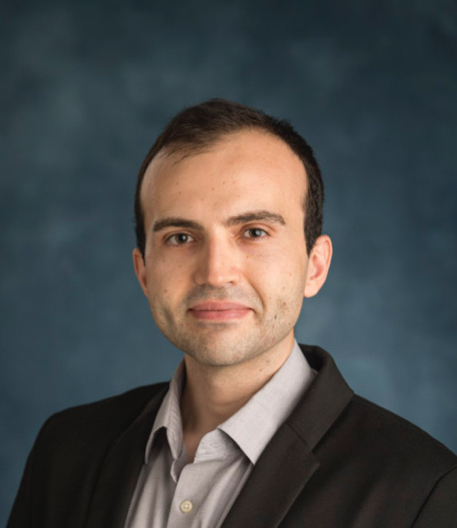
\includegraphics[width=0.2\linewidth]{assets/mert.jpg}
}

\titlegraphic{
\includegraphics[width=0.4\textwidth]{assets/SUSig_2color_Stree_Left.eps}}

\newcommand{\horizontalrule}{
	{
			\vspace{-0.5em}
			\center \rule{\textwidth}{0.1em}
			\vspace{-0.2em}
		}
}

\newcommand{\red}[1]{\textcolor{Red}{#1}}
\newcommand{\green}[1]{\textcolor{ForestGreen}{#1}}
\newcommand{\blue}[1]{\textcolor{DarkBlue}{#1}}
\newcommand{\purple}[1]{\textcolor{Magenta}{#1}}

%\logo{
\includegraphics[height=0.5cm]{assets/Block_S_2_color.eps}}

%\institute{Stanford University}
\date{}

\begin{document}

\maketitle
%% main content starts %%

\begin{frame}{Overview}

	{
		\large \red{Problem}: Training neural networks is slow and sensitive.
	}

	\pause
	\vspace{0.5em}
	\horizontalrule
	\vspace{0.5em}

	{
		\large \green{Our Contribution}: use convex reformulations for training.
	}

	\pause
	\vspace{0.5em}

	\begin{enumerate}
		\item \textbf{Equivalent Model Classes}: new convex reformulations of neural networks.\pause

		\item \textbf{Cone Decompositions}: new connections between our convex training programs.\pause

		\item \textbf{Algorithms}: robust, tuning-free, and fast algorithms leveraging these connections.
	\end{enumerate}

\end{frame}

\setbeamercolor{background canvas}{bg=LightCyan}

\begin{frame}{}
	\begin{center}
		\huge I. 10 Years of Neural Nets
	\end{center}
\end{frame}
\setbeamercolor{background canvas}{bg=white}

\begin{frame}{Context: Ten Years Since AlexNet}

	{
		\large \textbf{10 Years Ago}: AlexNet won ILSVRC 2012 and started the modern ``deep learning'' movement in ML.
	}
	\pause

	\vspace{1em}

	\horizontalrule

	\vspace{1em}

	AlexNet improved over the next best model by \( \approx 10\% \) (top-5).

	\vspace{1em}

	\textbf{Key Techniques}:
	\begin{itemize}
		\item ``a large, deep convolutional neural network''.
		\item ``a very efficient GPU implementation of convolutional nets''.
		\item ``'dropout', a recently-developed regularization method that proved to be very effective.''
	\end{itemize}

	\source{https://image-net.org/challenges/LSVRC/2012/results.html\#abstract}
\end{frame}

\begin{frame}{Context: ImageNet Today}

	\begin{center}
		\large AlexNet won with \( 84.69\% \) top-five accuracy \citep{krizhevsky2012alexnet}.
	\end{center}

	\pause
	\horizontalrule

	\begin{center}
		\large Today, models get \( 99.02\% \) top-5 accuracy \citep{yuan2021florence}!

		\vspace{3em}

		(Using all sorts of tricks like pre-training, transformers, etc.)
	\end{center}
\end{frame}


%\begin{frame}{Context: Slides from the Winners}
%    \begin{figure}[]
%        \centering
%        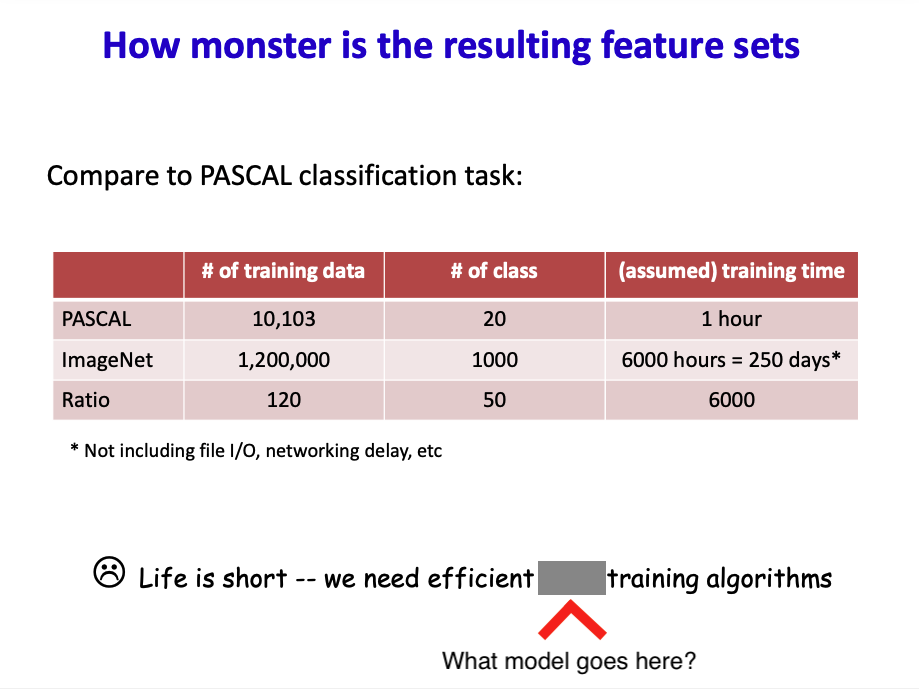
\includegraphics[width=0.9\textwidth]{assets/imagenet_2010_training_algos_grayed.png}
%    \end{figure}

%    \source{https://www.image-net.org/static\_files/files/ILSVRC2010\_NEC-UIUC.pdf}
%\end{frame}


%\begin{frame}{Context: Slides from the Winners --- Revealed!}
%    \begin{figure}[]
%        \centering
%        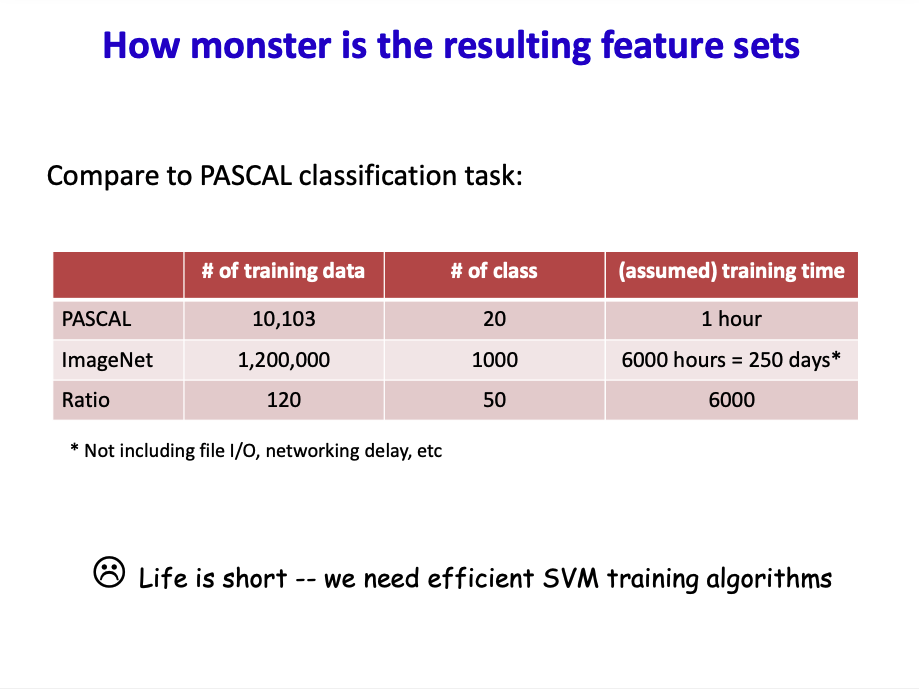
\includegraphics[width=0.9\textwidth]{assets/imagenet_2010_training_algos.png}
%    \end{figure}

%    \source{https://www.image-net.org/static\_files/files/ILSVRC2010\_NEC-UIUC.pdf}
%\end{frame}


\begin{frame}{Context: DALL$\cdot$E 2}

	\begin{figure}[]
		\centering
		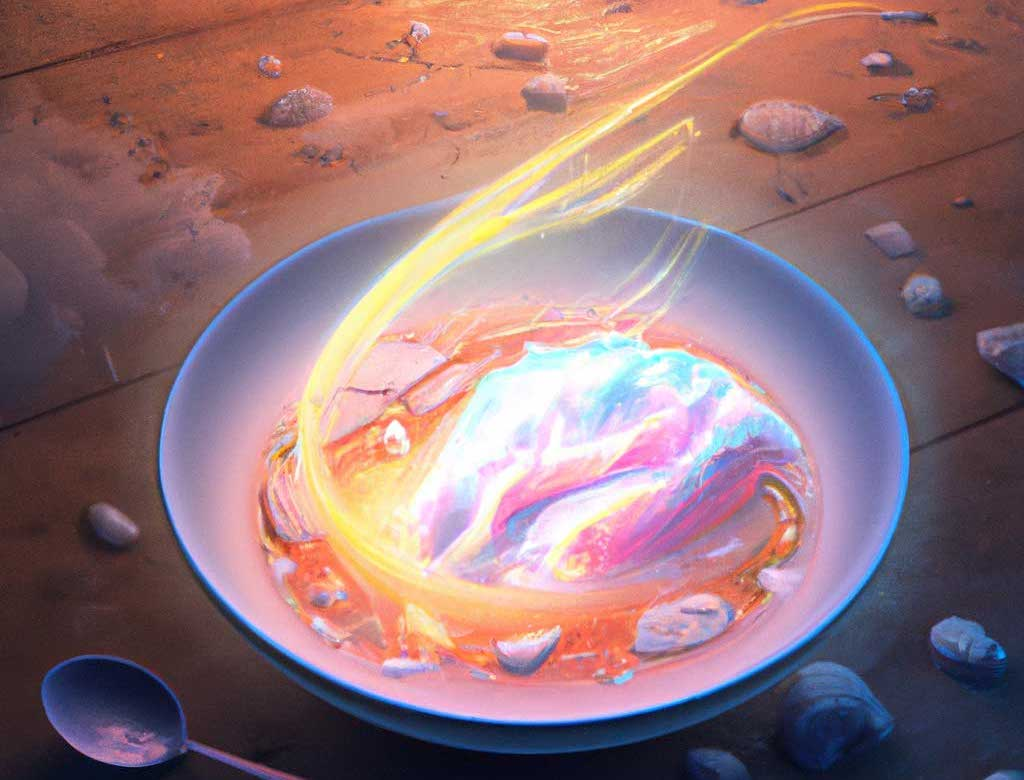
\includegraphics[width=0.65\linewidth]{assets/bowl_of_soup.jpg}
		\caption*{Generated by DALL$\cdot$E 2}%
	\end{figure}

	\begin{center}
		\textit{\Large A bowl of soup that is a portal to another
			dimension as digital art.}
	\end{center}

	\source{https://openai.com/dall-e-2/}

\end{frame}

\begin{frame}{Context: Cost of Training DALL$\cdot$E 2}

	\begin{center}
		\Large
		DALL$\cdot$E 2 has 5.5 billion parameters and took \red{billions} of Adam
		iterations to fit \citep{ramesh2022dalle}.
	\end{center}

	\pause
	\horizontalrule

	\begin{center}
		\Large
		\textbf{Main Challenge}: neural networks are \textcolor{red}{non-convex}.
	\end{center}


	\begin{figure}[]
		\centering
		%! TEX root = ../../main.tex
%% Illustration of step-sizes bound from Armijo line-search. 

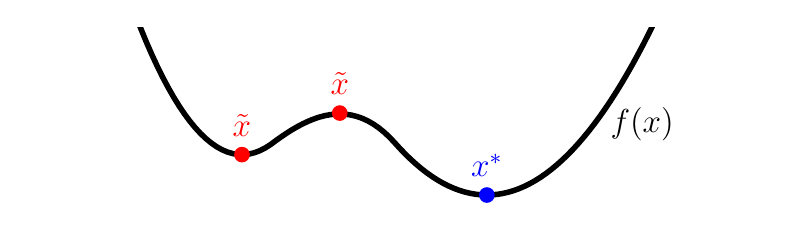
\begin{tikzpicture}[scale=1,
		declare function={
				objective(\x)=      (\x<=-1) * (2*\x*\x + 6*\x + 4)    +
				and(\x>-1, \x<=1) * (\x + 5 - pow(\x,3) - 5*\x*\x) / 4 +
				(\x>1) * (\x*\x - 5*\x + 4);
			}
	]
	\begin{axis}[
			width=0.9\textwidth,
			height=4cm,
			axis x line=none, axis y line=none,
			ymin=-3.25, ymax=5, ytick={-5,...,5}, ylabel=$y$,
			xmin=-5, xmax=7, xtick={-5,...,7}, xlabel=$x$,
		]

		\addplot[name path=function, domain=-3.5:5.23, samples=100, line width=2pt]{objective(x)};

        \node[label={[text=blue]90:$x^*$},circle,fill=blue,inner sep=2pt] at (axis cs:2.5,-2.25) {};
        \node[label={[text=red]90:$\tilde x$},circle,fill=red,inner sep=2pt] at (axis cs:0.09717,1.3) {};
        \node[label={[text=red]90:$\tilde x$},circle,fill=red,inner sep=2pt] at (axis cs:-1.5,-0.5) {};

		\node[label={0:$f(x)$}] at (axis cs:4.2,0.8) {};
	\end{axis}
\end{tikzpicture}


	\end{figure}

\end{frame}

\begin{frame}{Context: Challenges Optimizing Neural Networks}
	\begin{center}
		\Large
		Optimizing neural networks with SGD is \textcolor{red}{hard}!
	\end{center}

	\begin{itemize}
		\item \textbf{Tuning}: step-size, momentum, batch-size, etc.

		\item \textbf{Model Churn}: new seed, different
		      performance \citep{henderson2018deep}.

		\item \textbf{Certificates}: few/no guarantees.
	\end{itemize}

	\pause
	\horizontalrule

	\begin{center}
		\Large
		But these issues don't exist for convex models!
	\end{center}

	\begin{itemize}
		\item \textbf{Tuning}: line-search, full-batch methods, acceleration, etc.

		\item \textbf{Model Churn}: strict/strong convexity gives uniqueness.

		\item \textbf{Certificates}: stationary points are global minima.
	\end{itemize}


\end{frame}

\begin{frame}{Context: Practical Challenges}

	\begin{center}
		\large
		Recovering a two-layer ReLU network from data generated by a two-layer ReLU network.
	\end{center}

	\pause

	\begin{figure}[]
		\centering
		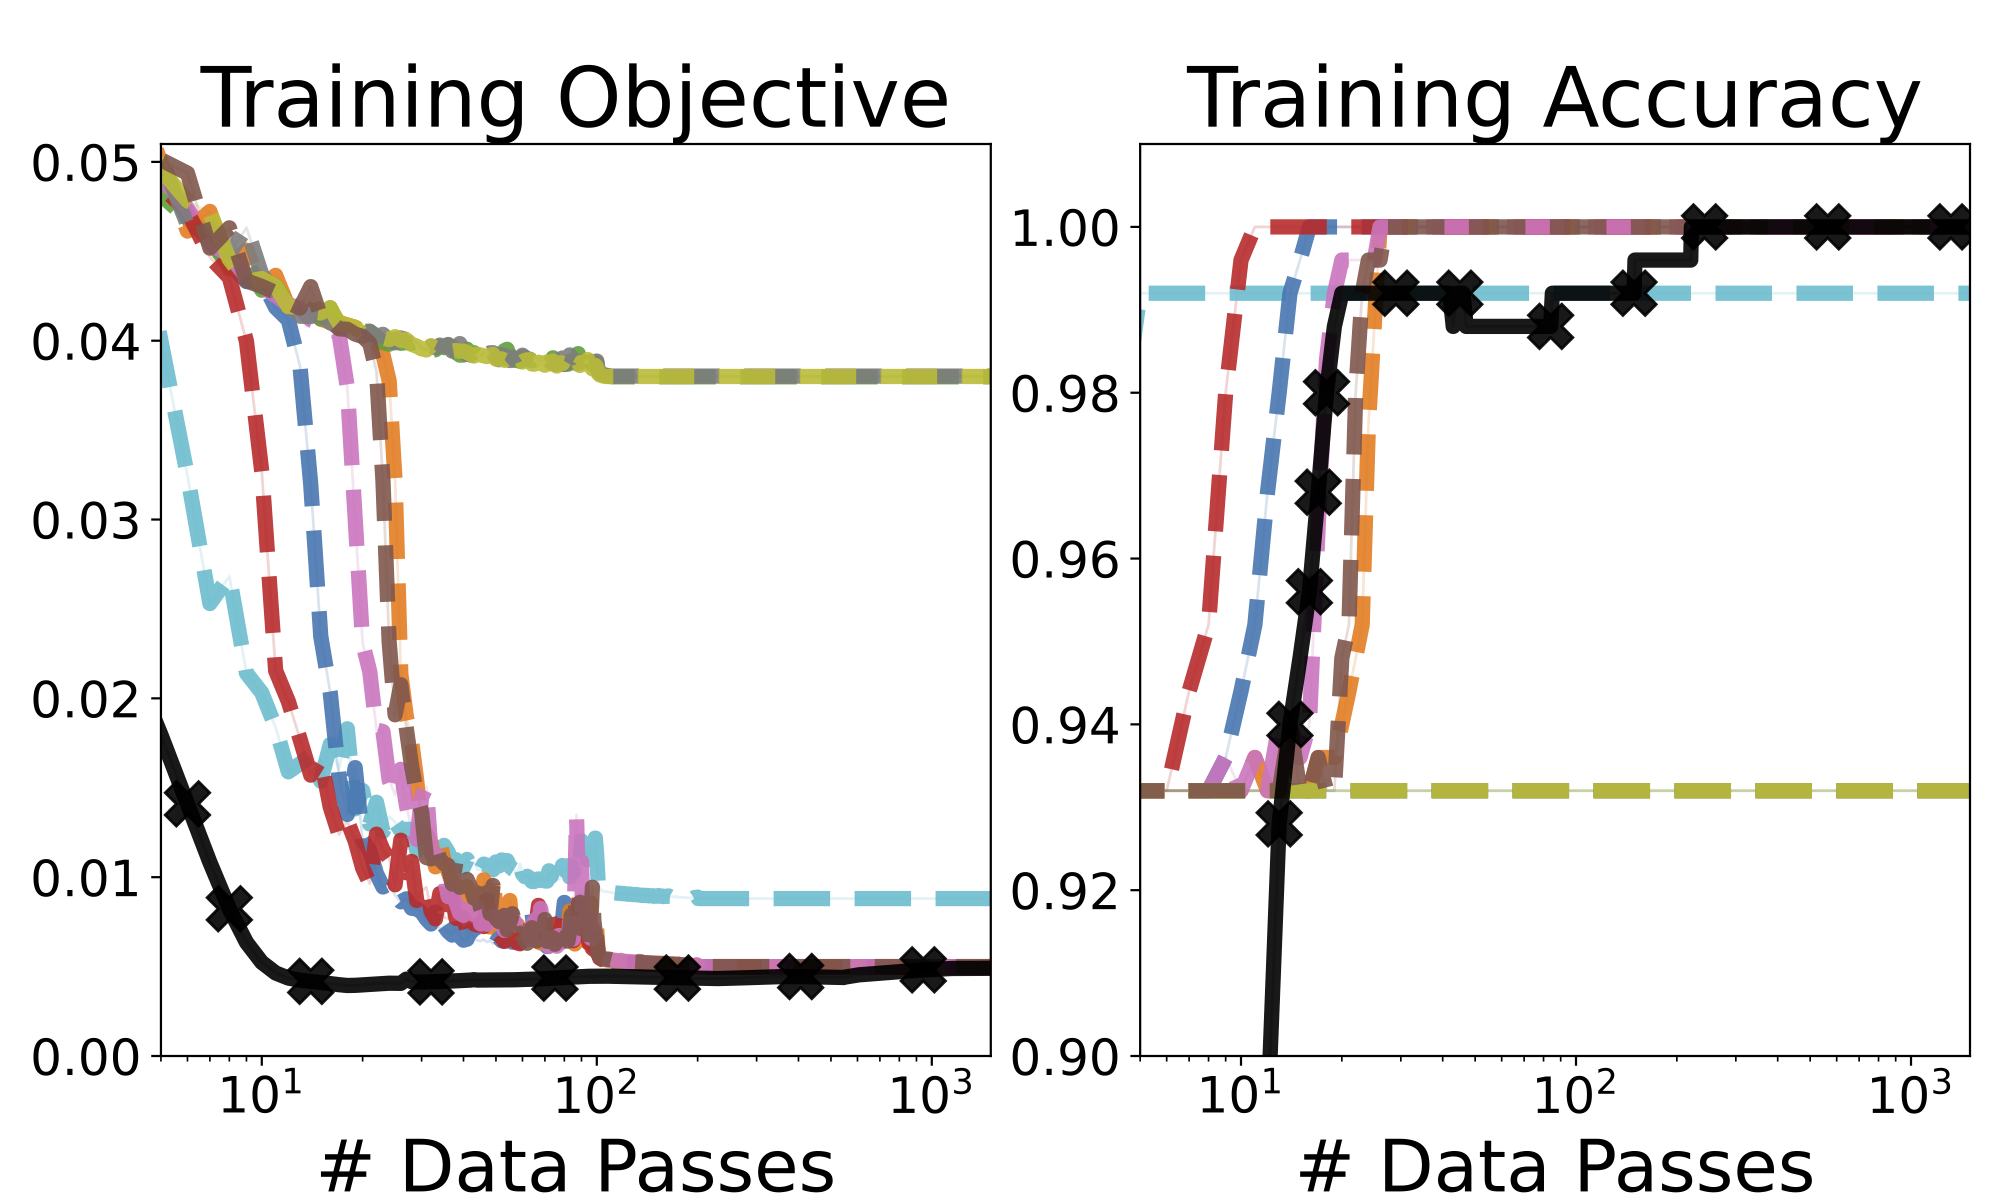
\includegraphics[width=0.9\textwidth]{assets/synthetic_classification.png}
	\end{figure}
\end{frame}

\begin{frame}{Context: Better Methods}
	\begin{center}
		{ \Large
			We need better methods!
		}

	\end{center}
	\vspace{1em}
	\pause

	\begin{itemize}
		\item \textbf{Stable} --- No mysterious failure modes.\pause

		      \vspace{0.5em}
		\item \textbf{Tuning-Free} --- No grid-search.\pause

		      \vspace{0.5em}
		\item \textbf{Robust} --- Work on a variety of problems.\pause

		      \vspace{0.5em}
		\item \textbf{Fast} --- better than \( O(1/\sqrt{T}) \).
	\end{itemize}
\end{frame}


\setbeamercolor{background canvas}{bg=LightCyan}

\begin{frame}{}
	\begin{center}
		\huge II. Equivalent (Convex) Model Classes
	\end{center}
\end{frame}
\setbeamercolor{background canvas}{bg=white}

\begin{frame}{Convex Reformulations: Flavor of Results}

	{ \large
		\textbf{Basic Idea}: We start with a \red{non-convex} optimization problem and derive
		an equivalent \green{convex} optimization problem.
	}

	\pause
	\vspace{2em}

	\textbf{Equivalent} means:
	\vspace{0.5em}
	\begin{itemize}
		\item The global minima have the same values: \( p^* = d^* \)
		      \vspace{0.5em}
		\item We can map a solution \( u^* \) for one problem into a solution
		      \( v^* \) for the other.
		      \vspace{0.5em}
		\item Call this our \emph{solution mapping}.
	\end{itemize}

\end{frame}


\begin{frame}{Convex Reformulations: Two-Layer ReLU Networks}

	{\large \textcolor{Red}{Non-Convex Problem}}
	\[
		\min_{w, \alpha} \underbrace{\norm{\sum_{j=1}^m (X w_j)_+ \alpha_j - y}_2^2}_{\text{Squared Error}}
		+ \underbrace{\lambda \sum_{j=1}^m \norm{w_j}_2^2 + |\alpha_j|^2}_{\text{Weight Decay}},
	\]
	where \( \rbr{x}_+ = \max\cbr{x, 0} \) is the ReLU activation.
	\pause

	\begin{figure}[]
		\centering
		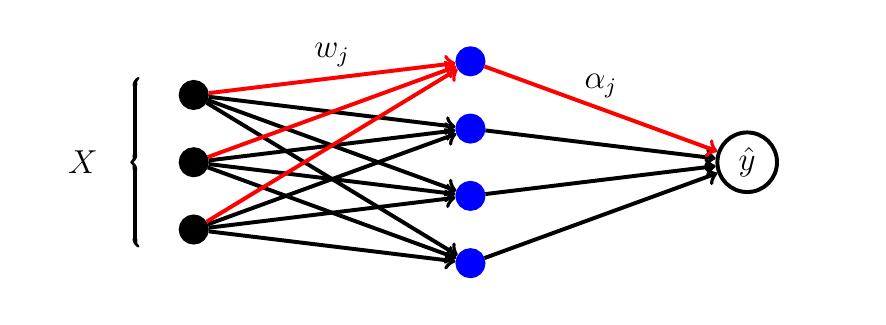
\begin{tikzpicture}[scale=1,
	]
	\begin{axis}[width=\linewidth, height=5cm,
			axis lines=none,  % don't print axis lines
			yticklabels={,,}, xticklabels={,,},
			ymin=0, ymax=8, y axis line style={-},
			xmin=0, xmax=15, x axis line style={-},
		]
		\node [] (input) at (axis cs:1,4) {$X$};
		\node [Input] (input1) at (axis cs:3,2) {};
		\node [Input] (input2) at (axis cs:3,4) {};
		\node [Input] (input3) at (axis cs:3,6) {};

		\draw [decorate, line width = 0.6mm,
			decoration = {calligraphic brace}] (axis cs:2,1.5) --  (axis cs:2,6.5);

		\node [Hidden] (hidden1) at (axis cs:8,1) {};
		\node [Hidden] (hidden2) at (axis cs:8,3) {};
		\node [Hidden] (hidden3) at (axis cs:8,5) {};
		\node [Hidden] (hidden4) at (axis cs:8,7) {};

		\draw [->, style=arrow, draw=black] (input1) -- (hidden1);
		\draw [->, style=arrow, draw=black] (input2) -- (hidden1);
		\draw [->, style=arrow, draw=black] (input3) -- (hidden1);

		\draw [->, style=arrow, draw=black] (input1) -- (hidden2);
		\draw [->, style=arrow, draw=black] (input2) -- (hidden2);
		\draw [->, style=arrow, draw=black] (input3) -- (hidden2);

		\draw [->, style=arrow, draw=black] (input1) -- (hidden3);
		\draw [->, style=arrow, draw=black] (input2) -- (hidden3);
		\draw [->, style=arrow, draw=black] (input3) -- (hidden3);

		\draw [->, style=arrow, draw=red] (input1) -- (hidden4);
		\draw [->, style=arrow, draw=red] (input2) -- (hidden4);
		\draw [->, style=arrow, draw=red] (input3) -- (hidden4) node[pos=0.5,above] {$w_{j}$};

		\node [Output] (output) at (axis cs:13,4) {$\hat y$};

		\draw [->, style=arrow, draw=black] (hidden1) -- (output);
		\draw [->, style=arrow, draw=black] (hidden2) -- (output);
		\draw [->, style=arrow, draw=black] (hidden3) -- (output);
		\draw [->, style=arrow, draw=red] (hidden4) -- (output) node[pos=0.5,above] {$\alpha_{j}$};
	\end{axis}

\end{tikzpicture}%

%\begin{tikzpicture}[scale=1,
%    ]
%    \begin{axis}[width=1.1\linewidth, height=5cm,
%            axis lines=none,  % don't print axis lines
%            yticklabels={,,}, xticklabels={,,},
%            ymin=-0.2, ymax=10.2, x axis line style={-},
%            xmin=-0.2, xmax=20.2, y axis line style={-},
%        ]

%        \filldraw[color=blue!60, fill=blue!5, line width=0.4mm](axis cs:0,5.8) rectangle (axis cs:20, 10);
%        \filldraw[color=red!60, fill=red!5, line width=0.4mm](axis cs:0,0) rectangle (axis cs:20, 4.2);

%        % non-convex models
%        \filldraw[line width=0.4mm, fill=white](axis cs:1,1) rectangle (axis cs:8, 3.2) node[pos=.5] {NC-GReLU};
%        \filldraw[line width=0.4mm, fill=white](axis cs:12,1) rectangle (axis cs:19, 3.2) node[pos=.5] {NC-ReLU};

%        % convex models
%        \filldraw[line width=0.4mm, fill=white](axis cs:1,6.8) rectangle (axis cs:8, 9) node[pos=.5] {C-GReLU};
%        \filldraw[line width=0.4mm, fill=white](axis cs:12,6.8) rectangle (axis cs:19, 9) node[pos=.5] {C-ReLU};

%        \draw [<->, solid, draw=black, line width = 0.6mm] (axis cs:4.5,3.2) -- (axis cs:4.5,6.8) node[right, pos=0.5] {\small Sol. Map};

%        \draw [<->, solid, draw=black, line width = 0.6mm] (axis cs:15.5,3.2) -- (axis cs:15.5,6.8)  node[right, pos=0.5] {\small Sol. Map};

%        \draw [<-, solid, draw=black, line width = 0.6mm] (axis cs:6,9) -- [bend left=15] (axis cs:14, 9);

%        \draw [->, solid, draw=orange, line width = 0.6mm] (axis cs:8,7.9) -- (axis cs:12,7.9);
%        \node[align=center] at (axis cs:10.1, 7.8) {\small Cone\\ \small Decomp.};
%    \end{axis}

%\end{tikzpicture}%


	\end{figure}

\end{frame}
\begin{frame}{Convex Reformulations: Convex Problem}

	{\large \textcolor{ForestGreen}{Convex Reformulation}} \citep{pilanci2020convex}
	\[
		\begin{aligned}
			\min_{u} & \norm{\sum_{j=1}^p D_j X (v_j - w_j) - y}_2^2 +
			\lambda \sum_{j=1}^p \norm{v_j}_2 + \norm{w_j}_2           \\
			         & \hspace{0.2em} \text{s.t. }
			v_j, w_j \in \calK_j := \cbr{w : (2D_j - I) X w \geq 0},
		\end{aligned}
	\]
	where \( D_j = \text{diag}[\mathbbm{1}(X g_j \geq 0)] \).
	\pause

	\begin{figure}[]
		\centering
		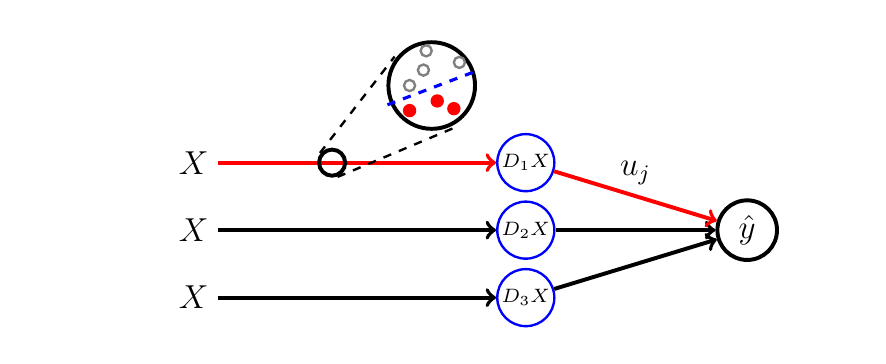
\begin{tikzpicture}[scale=1,
	]
	\begin{axis}[width=\linewidth, height=5.5cm,
			axis lines=none,  % don't print axis lines
			yticklabels={,,}, xticklabels={,,},
			ymin=0, ymax=8, y axis line style={-},
			xmin=0, xmax=15, x axis line style={-},
		]
		\node [] (input1) at (axis cs:3,1) {$X$};
		\node [] (input2) at (axis cs:3,2.75) {$X$};
		\node [] (input3) at (axis cs:3,4.5) {$X$};

        \node [Splits] (hidden1) at (axis cs:9,1) {\scriptsize $D_3 X$};
		\node [Splits] (hidden2) at (axis cs:9,2.75) {\scriptsize $D_2 X$};
		\node [Splits] (hidden3) at (axis cs:9,4.5) {\scriptsize $D_1 X$};

		\draw [->, style=arrow, draw=black] (input1) -- (hidden1);

		\draw [->, style=arrow, draw=black] (input2) -- (hidden2);

		\draw [->, style=arrow, draw=red] (input3) -- (hidden3);

		\node [Output] (output) at (axis cs:13,2.75) {$\hat y$};

		\draw [->, style=arrow, draw=black] (hidden1) -- (output);
		\draw [->, style=arrow, draw=black] (hidden2) -- (output);
		\draw [->, style=arrow, draw=red] (hidden3) -- (output) node[pos=0.5,above] {$u_j$};

		\draw [draw=black, line width=0.3mm, dashed] (axis cs:5.6, 4.13) -- (axis cs:7.7,5.4);
		\draw [draw=black, line width=0.3mm, dashed] (axis cs:5.28, 4.75) -- (axis cs:6.63,7.25);

		\node [draw=black, minimum size=0.3cm, shape=circle, solid, line width=0.5mm] (examine) at (axis cs:5.5,4.5) {};
		\node [draw=black, minimum size=1.1cm, shape=circle, solid, line width=0.5mm] (closeup) at (axis cs:7.3,6.5) {};

		\node [fill=white, draw=gray, line width=0.3mm, inner sep=0.05cm, shape=circle] at (axis cs:7.8,7.1) {};
		\node [fill=white, draw=gray, line width=0.3mm, inner sep=0.05cm, shape=circle] at (axis cs:7.15,6.9) {};
		\node [fill=white, draw=gray, line width=0.3mm, inner sep=0.05cm, shape=circle] at (axis cs:7.2,7.4) {};
		\node [fill=white, draw=gray, line width=0.3mm, inner sep=0.05cm, shape=circle] at (axis cs:6.9,6.5) {};

		\draw [draw=Blue, dashed, line width=0.4mm] (axis cs:6.5,6.) -- (axis cs:8.15,6.9);

		\node [fill=Red, inner sep=0.06cm, shape=circle] at (axis cs:6.9,5.85) {};
		\node [fill=Red, inner sep=0.06cm, shape=circle] at (axis cs:7.4,6.1) {};
		\node [fill=Red, inner sep=0.06cm, shape=circle] at (axis cs:7.7,5.9) {};

	\end{axis}

\end{tikzpicture}%

%\begin{tikzpicture}[scale=1,
%    ]
%    \begin{axis}[width=1.1\linewidth, height=5cm,
%            axis lines=none,  % don't print axis lines
%            yticklabels={,,}, xticklabels={,,},
%            ymin=-0.2, ymax=10.2, x axis line style={-},
%            xmin=-0.2, xmax=20.2, y axis line style={-},
%        ]

%        \filldraw[color=blue!60, fill=blue!5, line width=0.4mm](axis cs:0,5.8) rectangle (axis cs:20, 10);
%        \filldraw[color=red!60, fill=red!5, line width=0.4mm](axis cs:0,0) rectangle (axis cs:20, 4.2);

%        % non-convex models
%        \filldraw[line width=0.4mm, fill=white](axis cs:1,1) rectangle (axis cs:8, 3.2) node[pos=.5] {NC-GReLU};
%        \filldraw[line width=0.4mm, fill=white](axis cs:12,1) rectangle (axis cs:19, 3.2) node[pos=.5] {NC-ReLU};

%        % convex models
%        \filldraw[line width=0.4mm, fill=white](axis cs:1,6.8) rectangle (axis cs:8, 9) node[pos=.5] {C-GReLU};
%        \filldraw[line width=0.4mm, fill=white](axis cs:12,6.8) rectangle (axis cs:19, 9) node[pos=.5] {C-ReLU};

%        \draw [<->, solid, draw=black, line width = 0.6mm] (axis cs:4.5,3.2) -- (axis cs:4.5,6.8) node[right, pos=0.5] {\small Sol. Map};

%        \draw [<->, solid, draw=black, line width = 0.6mm] (axis cs:15.5,3.2) -- (axis cs:15.5,6.8)  node[right, pos=0.5] {\small Sol. Map};

%        \draw [<-, solid, draw=black, line width = 0.6mm] (axis cs:6,9) -- [bend left=15] (axis cs:14, 9);

%        \draw [->, solid, draw=orange, line width = 0.6mm] (axis cs:8,7.9) -- (axis cs:12,7.9);
%        \node[align=center] at (axis cs:10.1, 7.8) {\small Cone\\ \small Decomp.};
%    \end{axis}

%\end{tikzpicture}%


	\end{figure}
\end{frame}

\begin{frame}{Convex Reformulations: Breaking it Down}

	\[
		\begin{aligned}
			\min_{u} & \norm{\sum_{j=1}^p D_j X (v_j - w_j) - y}_2^2 +
			\lambda \sum_{j=1}^p \norm{v_j}_2 + \norm{w_j}_2           \\
			         & \hspace{0.2em} \text{s.t. }
			v_j, w_j \in \calK_j := \cbr{w : (2D_j - I) X w \geq 0},
		\end{aligned}
	\]
	where \( \purple{D_j = \text{diag}[\mathbbm{1}(X g_j \geq 0)]} \).

	\horizontalrule

	\begin{itemize}
		\item \purple{\( D_j \) is a ReLU activation pattern induced by ``gate'' \( g_j \).}
		      \pause
		      \begin{itemize}
			      \item \([D_j]_{ii} = 1\) if \( \abr{x_i, g_i} \geq 0 \) and \( 0 \) otherwise.
		      \end{itemize}

	\end{itemize}
	\vspace{7.3em}
\end{frame}

\begin{frame}{Convex Reformulations: Breaking it Down}

	\[
		\begin{aligned}
			\min_{u} & \norm{\sum_{j=1}^p D_j X (v_j - w_j) - y}_2^2 +
			\purple{\lambda \sum_{j=1}^p \norm{v_j}_2 + \norm{w_j}_2}  \\
			         & \hspace{0.2em} \text{s.t. }
			v_j, w_j \in \calK_j := \cbr{w : (2D_j - I) X w \geq 0}
		\end{aligned}
	\]
	where \( D_j = \text{diag}[\mathbbm{1}(X g_j \geq 0)] \).

	\horizontalrule

	\begin{itemize}
		\item \( D_j \) is a ReLU activation pattern induced by ``gate'' \( g_j \).
		      \begin{itemize}
			      \item \([D_j]_{ii} = 1\) if \( \abr{x_i, g_i} \geq 0 \) and \( 0 \) otherwise.
		      \end{itemize}
		\item \purple{Weight-decay regularization turns into ``group \( \ell_1 \)'' penalty.}
	\end{itemize}
	\vspace{6em}
\end{frame}

\begin{frame}{Convex Reformulations: Breaking it Down}

	\[
		\begin{aligned}
			\min_{u} & \norm{\sum_{j=1}^p D_j X (v_j - w_j) - y}_2^2 +
			\lambda \sum_{j=1}^p \norm{v_j}_2 + \norm{w_j}_2           \\
			         & \hspace{0.2em} \purple{\text{s.t. }
				v_j, w_j \in \calK_j := \cbr{w : (2D_j - I) X w \geq 0},}
		\end{aligned}
	\]
	where \( D_j = \text{diag}[\mathbbm{1}(X g_j \geq 0)] \).

	\horizontalrule

	\begin{itemize}
		\item \( D_j \) is a ReLU activation pattern induced by ``gate'' \( g_j \).
		      \begin{itemize}
			      \item \([D_j]_{ii} = 1\) if \( \abr{x_i, g_i} \geq 0 \) and \( 0 \) otherwise.
		      \end{itemize}
		\item Weight-decay regularization turns into ``group \( \ell_1 \)'' penalty.
		\item \purple{The constraint \( v_j \in \calK_j \) implies
			      \[
				      \rbr{X v_j}_+ = D_j X v_j.
			      \]
			      That is, \( v_j \) has the activation encoded by \( D_j \).
		      }
	\end{itemize}
\end{frame}

\begin{frame}{Convex Reformulations: Hardness}


	\[
		p = \abs{\cbr{D_j = \text{diag}[\mathbbm{1}(X g_j \geq 0)] : g_j \in \R^d }}
	\]

	\vspace{2em}
	\pause

	The \textbf{convex program} is:
	\vspace{0.5em}
	\begin{itemize}
		\item \red{Exponential in general}: \( p \in O(r \cdot (\frac{n}{r})^r) \),
		      where \( r = \text{rank}(X) \).
		      \vspace{0.25em}
		      \begin{itemize}
			      \item Bound comes from theory of hyperplane arrangements \citep{winder1966partitions}.
		      \end{itemize}
		      \pause

		      \vspace{0.5em}

		\item Highly \green{structured} --- it's a (constrained) generalized linear model!
	\end{itemize}

	\vspace{1em}
	\pause

	\begin{center}
		\Large
		We exchange one kind of hardness for another.
	\end{center}

\end{frame}


\begin{frame}{Convex Reformulations: Big Picture}

	\begin{figure}[]
		\centering
		%! TEX root = ../../main.tex

%% illustration of relations between hypothesis classes. 

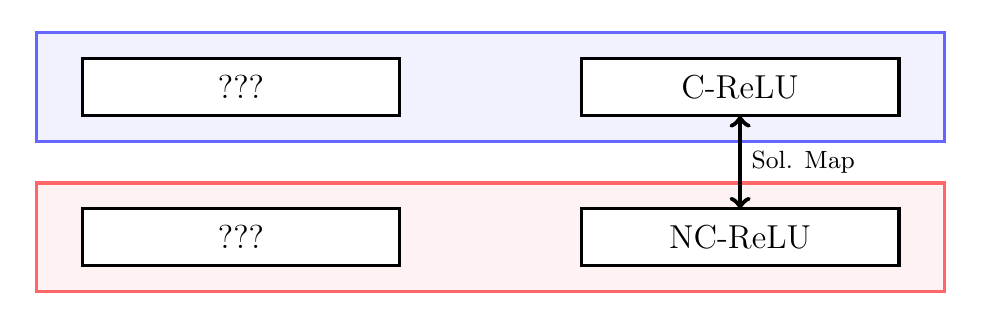
\begin{tikzpicture}[scale=1,
	]
	\begin{axis}[width=1.1\linewidth, height=5cm,
			axis lines=none,  % don't print axis lines
			yticklabels={,,}, xticklabels={,,},
			ymin=-0.2, ymax=10.2, x axis line style={-},
			xmin=-0.2, xmax=20.2, y axis line style={-},
		]

		\filldraw[color=blue!60, fill=blue!5, line width=0.4mm](axis cs:0,5.8) rectangle (axis cs:20, 10);
		\filldraw[color=red!60, fill=red!5, line width=0.4mm](axis cs:0,0) rectangle (axis cs:20, 4.2);

		% non-convex models
		\filldraw[line width=0.4mm, fill=white](axis cs:1,1) rectangle (axis cs:8, 3.2) node[pos=.5] {???};
		\filldraw[line width=0.4mm, fill=white](axis cs:12,1) rectangle (axis cs:19, 3.2) node[pos=.5] {NC-ReLU};

		% convex models
		\filldraw[line width=0.4mm, fill=white](axis cs:1,6.8) rectangle (axis cs:8, 9) node[pos=.5] {???};
		\filldraw[line width=0.4mm, fill=white](axis cs:12,6.8) rectangle (axis cs:19, 9) node[pos=.5] {C-ReLU};

		\draw [<->, solid, draw=black, line width = 0.6mm] (axis cs:15.5,3.2) -- (axis cs:15.5,6.8)  node[right, pos=0.5] {\small Sol. Map};

	\end{axis}

\end{tikzpicture}%

	\end{figure}

\end{frame}


\begin{frame}{Convex Reformulations: Unconstrained Relaxation}
	What can we do with the convex ReLU problem?

	\[
		\begin{aligned}
			\textbf{C-ReLU}: \min_{u} & \norm{\sum_{j=1}^p D_j X (v_j - w_j) - y}_2^2 +
			\lambda \sum_{j=1}^p \norm{v_j}_2 + \norm{w_j}_2                            \\
			                          & \hspace{0.2em} \red{\text{s.t. }
				v_j, w_j \in \calK_j := \cbr{w : (2D_j - I) X w \geq 0},}
		\end{aligned}
	\]

	\pause
	\horizontalrule

	\textbf{Relaxation}: drop the cone constraints and simplify to obtain,
	\[
		\begin{aligned}
			\textbf{C-GReLU}: \min_{u} & \norm{\sum_{j=1}^p D_j X u_j - y}_2^2 +
			\lambda \sum_{j=1}^p \norm{u_j}_2                                    \\
		\end{aligned}
	\]

	\pause
	\red{What does it mean? Is it a neural network still?}
\end{frame}


\begin{frame}{Convex Reformulations: Gated ReLU Networks}

	\begin{beamercolorbox}[wd=\textwidth,sep=1em]{result}
		\textbf{Theorem 2.2} (informal): C-GReLU is equivalent to solving
		\[
			\textbf{NC-GReLU}: \min_{W_1, \alpha} \half \norm{\sum_{j=1}^p \phi_{g_j}(X, w_{j})\alpha - y}_2^2 + \frac{\lambda}{2} \sum_{j=1}^p \norm{w_{j}}_2^2 + |\alpha_j|^2,
		\]
		with the ``Gated ReLU'' \citep{fiat2019decoupling} activation function
		\[ \phi_{g}(X, u) = \text{diag}(\mathbbm{1}(Xg \geq 0)) X u, \]
		and gate vectors \( g_j \) such that
		\[
			D_j = \text{diag}[\mathbbm{1}(X g_j \geq 0).
		\]
	\end{beamercolorbox}
	\pause

	\textbf{Interpretation}: if \( u_j \not \in \calK_j \), then the activation
	must be decoupled from the linear mapping in the non-convex model.

\end{frame}

\begin{frame}{Gated ReLU Networks: Proof Sketch}
	The proof reduces C-GReLU to NC-GReLU and vice-versa.

	\vspace{1em}

	\textbf{Roadmap}:
	\begin{enumerate}
		\item Manipulate NC-GReLU to remove invariance to certain
		      scale re-parameterizations.
		\item Merge second-layer weights into first-layer weights.
	\end{enumerate}

	\pause
	\horizontalrule

	The prediction function is
	\[
		\begin{aligned}
			f_{w, \alpha}(X) & = \sum_{j=1}^p \phi_{g_j}(X, w_{j})\alpha                                  \\\pause
			                 & = \sum_{j=1}^p \text{diag}(\mathbbm{1}(Xg_j \geq 0)) X w_j \cdot \alpha_j.
		\end{aligned}
	\]
	\pause
	Invariant to scale re-parameterizations of the form
	\[
		w'_j = w_j \cdot \beta, \quad \alpha_j' = \frac{\alpha_j}{\beta_j}.
	\]
\end{frame}

\begin{frame}{Gated ReLU Networks: Sketch Continued}
	Let \purple{\( \rbr{w^*, \alpha^*} \)} be a solution to NC-GReLU.\pause

	\vspace{1em}
	By Young's inequality,
	\[
		2 \sum_{j=1}^p \norm{w_j^*}_2 \abs{\alpha_j^*} \leq \sum_{j=1}^p \norm{w_j^*}_2^2 + |\alpha^*_j|^2
	\]\pause
	Equality is achieved for \( w'_j = w_j^* \cdot \beta \), \( \alpha_j' = \alpha_j^* / \beta \), where
	\[ \purple{\beta = \sqrt{\frac{|\alpha_j^*|}{\norm{w_j^*}_2}}.} \]
	\pause
	But \( f \) is invariant to such re-parameterizations!
	\pause
	\begin{align*}
		\half & \norm{\sum_{j=1}^p \phi_{g_j}(X, w^*_{j})\alpha_j^* - y}_2^2 + \frac{\lambda}{2} \sum_{j=1}^p \norm{w^*_{j}}_2^2 + |\alpha_j^*|^2    \\
		      & \quad \quad \geq \half \norm{\sum_{j=1}^p \phi_{g_j}(X, w'_{j})\alpha'_j - y}_2^2 + \lambda \sum_{j=1}^p \norm{w'_{j}}_2 |\alpha'_j| \\
	\end{align*}
\end{frame}

\begin{frame}{Gated ReLU Networks: Sketch Continued}
	Now we use positive homogeneity of the norm,
	\[
		\begin{aligned}
			\half & \norm{\sum_{j=1}^p \phi_{g_j}(X, w'_{j})\alpha'_j - y}_2^2 + \lambda \sum_{j=1}^p \norm{w'_{j}}_2|\alpha'_j|                                     \\
			      & \quad \quad = \half \norm{\sum_{j=1}^p \phi_{g_j}(X, w'_{j}\cdot\alpha'_j) - y}_2^2 + \lambda \sum_{j=1}^p \norm{w'_{j} \cdot |\alpha'_j|}_2     \\ \pause
			      & \quad \quad = \half \norm{\sum_{j=1}^p \phi_{g_j}(X, w''_{j}) - y}_2^2 + \lambda \sum_{j=1}^p \norm{w''_{j}}_2                                   \\ \pause
			      & \quad \quad \geq \min_{w} \half \norm{\sum_{j=1}^p \phi_{g_j}(X, w_{j}) - y}_2^2 + \lambda \sum_{j=1}^p \norm{w_{j}}_2 \quad (\textbf{C-GReLU}).
		\end{aligned}
	\]
	This completes the sketch.
\end{frame}

\begin{frame}{Gated ReLu Networks: Big Picture}
	\begin{center}
		\Large What do we do with these models?
	\end{center}

	\pause

	\begin{figure}[]
		\centering
		%! TEX root = ../../main.tex

%% illustration of relations between hypothesis classes. 

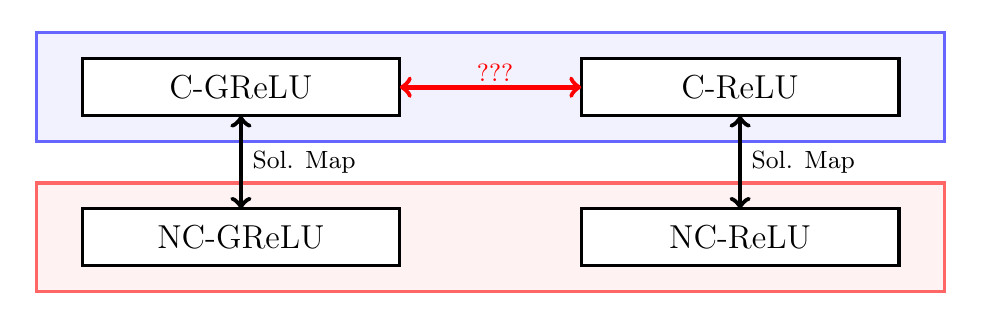
\begin{tikzpicture}[scale=1,
	]
	\begin{axis}[width=1.1\linewidth, height=5cm,
			axis lines=none,  % don't print axis lines
			yticklabels={,,}, xticklabels={,,},
			ymin=-0.2, ymax=10.2, x axis line style={-},
			xmin=-0.2, xmax=20.2, y axis line style={-},
		]

		\filldraw[color=blue!60, fill=blue!5, line width=0.4mm](axis cs:0,5.8) rectangle (axis cs:20, 10);
		\filldraw[color=red!60, fill=red!5, line width=0.4mm](axis cs:0,0) rectangle (axis cs:20, 4.2);

		% non-convex models
		\filldraw[line width=0.4mm, fill=white](axis cs:1,1) rectangle (axis cs:8, 3.2) node[pos=.5] {NC-GReLU};
		\filldraw[line width=0.4mm, fill=white](axis cs:12,1) rectangle (axis cs:19, 3.2) node[pos=.5] {NC-ReLU};

		% convex models
		\filldraw[line width=0.4mm, fill=white](axis cs:1,6.8) rectangle (axis cs:8, 9) node[pos=.5] {C-GReLU};
		\filldraw[line width=0.4mm, fill=white](axis cs:12,6.8) rectangle (axis cs:19, 9) node[pos=.5] {C-ReLU};

		\draw [<->, solid, draw=black, line width = 0.6mm] (axis cs:4.5,3.2) -- (axis cs:4.5,6.8) node[right, pos=0.5] {\small Sol. Map};

		\draw [<->, solid, draw=black, line width = 0.6mm] (axis cs:15.5,3.2) -- (axis cs:15.5,6.8)  node[right, pos=0.5] {\small Sol. Map};

		%\draw [<-, solid, draw=black, line width = 0.6mm] (axis cs:6,9) to [bend left=15] (axis cs:14, 9);

		\draw [<->, solid, draw=red, line width = 0.6mm] (axis cs:8,7.9) -- (axis cs:12,7.9);
		\node[align=center] at (axis cs:10.1, 7.8) {\small \red{???} \\};
	\end{axis}

\end{tikzpicture}%

	\end{figure}
\end{frame}


\setbeamercolor{background canvas}{bg=LightCyan}
\begin{frame}{}
	\begin{center}
		\huge III. Cone Decompositions
	\end{center}
\end{frame}
\setbeamercolor{background canvas}{bg=white}

\begin{frame}{Cone Decompositions: Gated ReLU Networks }

	\begin{center}
		\textbf{Question}: when are Gated ReLU and ReLU networks equivalent?
	\end{center}

	\pause
	\horizontalrule

	Consider special case where \( \lambda = 0 \).

	\[
		\textbf{C-GReLU}: \min_{u} \norm{\sum_{j=1}^p D_j X u_j - y}_2^2. \hspace{11em}
	\]
	\vspace{-1em}

	\begin{center}
		\Large \red{V.S.}
	\end{center}

	\vspace{-2em}
	\[
		\begin{aligned}
			\textbf{C-ReLU}: \min_{u} & \norm{\sum_{j=1}^p D_j X (v_j - w_j) - y}_2^2. \\
			                          & \hspace{0.2em} \text{s.t. }
			v_j, w_j \in \calK_j := \cbr{w : (2D_j - I) X w \geq 0},
		\end{aligned}
	\]

\end{frame}

\begin{frame}{Cone Decompositions: Equivalent Statement}

	\red{Equiv. Question}: when does \( u_j = v_j - w_j \) for some \( v_j, w_j \in \calK_j \)?

	\pause
	\vspace{1em}

	\green{Answer}: when \( \calK_j - \calK_j = \R^d \) and a ``cone decomposition'' exists.
	\pause

	\begin{figure}[]
		\centering
		%! TEX root = ../../main.tex

%% Illustration of cone decomposition. 

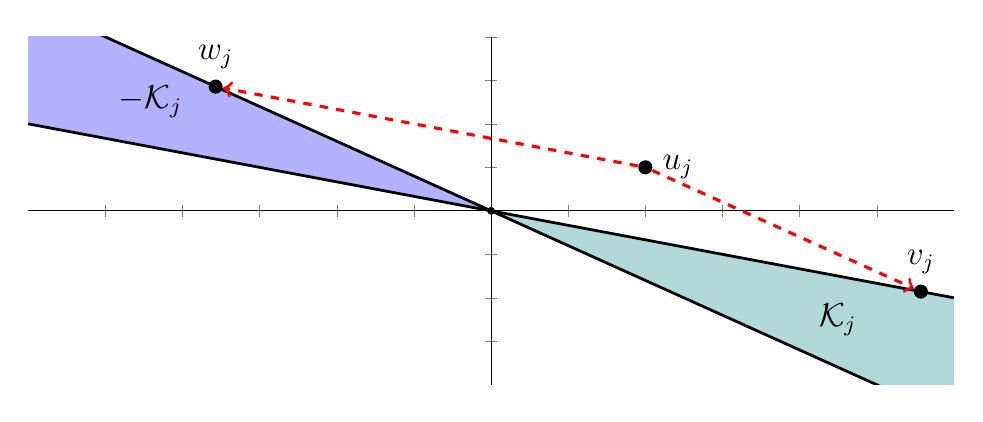
\begin{tikzpicture}[scale=1,
		declare function={
				cone_u(\x)= -\x/3;
				cone_l(\x)= -4*\x/5;
			}
	]
	\begin{axis}[width=1.1\linewidth, height=6cm,
			axis lines=center, yticklabels={,,}, xticklabels={,,},
			ymin=-4, ymax=4, ytick={-5,...,5}, ylabel=$$, x axis line style={-},
				xmin=-6, xmax=6, xtick={-5,...,5}, xlabel=$$, y axis line style={-},
		]
		\addplot[name path=cone_u, domain=-6:6, samples=100, line width=1pt]{cone_u(x)};
		\addplot[name path=cone_l, domain=-6:6, samples=200, line width=1pt]{cone_l(x)};

		% add color fill to both cones.
		\addplot fill between[
				of = cone_u and cone_l,
				split, % calculate segments
				every even segment/.style = {fill=blue, fill opacity=0.3},
				every odd segment/.style  = {fill=teal, fill opacity=0.3}
			];

		%% point labels
		% origin point
		\node[circle, fill, inner sep=1pt] at (axis cs:0,0) {};

		\node[label={0:$u_j$}, circle, fill, inner sep=1.8pt] (u) at (axis cs:2,1) {};
		\node[label={90:$v_j$}, circle, fill, inner sep=1.8pt] (v) at (axis cs:25/7+2, -25/21 - 2/3) {};
		\node[label={90:$w_j$}, circle, fill, inner sep=1.8pt] (w) at (axis cs:-25/7, 20/7) {};

		% labels
		\node[label={0:$\calK_j$}] at (axis cs:4,-2.5) {};
		\node[label={180:$-\calK_j$}] at (axis cs:-3.75,2.5) {};

		% lines
		\draw [->, dashed, draw=red, line width = 0.4mm] (u) edge (w);
		\draw [->, dashed, draw=red, line width = 0.4mm] (u) edge (v);
	\end{axis}

\end{tikzpicture}%

	\end{figure}

\end{frame}
\begin{frame}{Cone Decomposition: Basic Result}

	\textbf{Recall}: \( \calK_j = \cbr{w : (2 D_j - I) X w \geq 0} \).
	\pause

	\begin{itemize}
		\item This is a polyhedral cone which we rewrite as
		      \[
			      \calK_j = \bigcap_{i=1}^n \cbr{w : [S_j]_{ii} \cdot \abr{x, w} \geq 0},
		      \]
		      where \( S_j = (2D_j - I) \).
	\end{itemize}

	\pause
	\horizontalrule

	\begin{beamercolorbox}[wd=\textwidth,sep=1em]{result}
		\textbf{Proposition 3.1} (informal): If \( X \) is full row-rank,
		then \( \text{aff}(\calK_j) = \R^d \) and
		\( \calK_j - \calK_j = \R^d \).
	\end{beamercolorbox}

	\vspace{1em}

	\pause
	Unfortunately, there is no extension to full-rank \( X \).

\end{frame}

\begin{frame}{Cone Decompositions: Not All Cones are Equal}

	\textbf{Alternative Program}: show we don't need ``singular'' cones \( \calK_j \),
	\[
		\calK_j - \calK_j \subsetneq \R^d.
	\]

	\vspace{1em}
	\pause

	\begin{beamercolorbox}[wd=\textwidth,sep=1em]{result}
		\textbf{Proposition 3.2} (informal): Suppose \( \calK_j - \calK_j \subset \R^d \).
		Then, there exists \( \calK_i \) for which \( \calK_i - \calK_i = \R^d \)
		and \( \calK_j \subset \calK_i \).
	\end{beamercolorbox}

	\pause
	\vspace{1em}

	\textbf{Interpretation}: if optimal \( u^*_j \neq 0 \), then set
	\[
		u_i' = u_j^* + u_i^*.
	\]
	It is possible to show this causes no problems.


\end{frame}

\begin{frame}{Cone Decompositions: Proof Sketch}

	\textbf{Proof}: Works by iteratively constructing \( \calK_i \) s.t. \( \calK_j \subset \calK_i \).

	\pause
	\horizontalrule

	We sketch a simpler statement:

	\vspace{1em}

	\begin{beamercolorbox}[wd=\textwidth,sep=1em]{relaxation}
		\textbf{Proposition 3.2} (informal): Suppose \( \calK_j = \cbr{0} \).
		Then, there exists \( \calK_i \) for which \( \calK_i - \calK_i = \R^d \)
		and \( \calK_j \subset \calK_i \).
	\end{beamercolorbox}


\end{frame}


\begin{frame}{Cone Decompositions: Proof Sketch}
	\[
		\calK_j' = \cbr{w : [S_j]_{11} \cdot \abr{x_1, w} \geq 0}
	\]
	\begin{figure}[]
		\centering
		%! TEX root = ../../main.tex

%% Illustration of cone decomposition. 

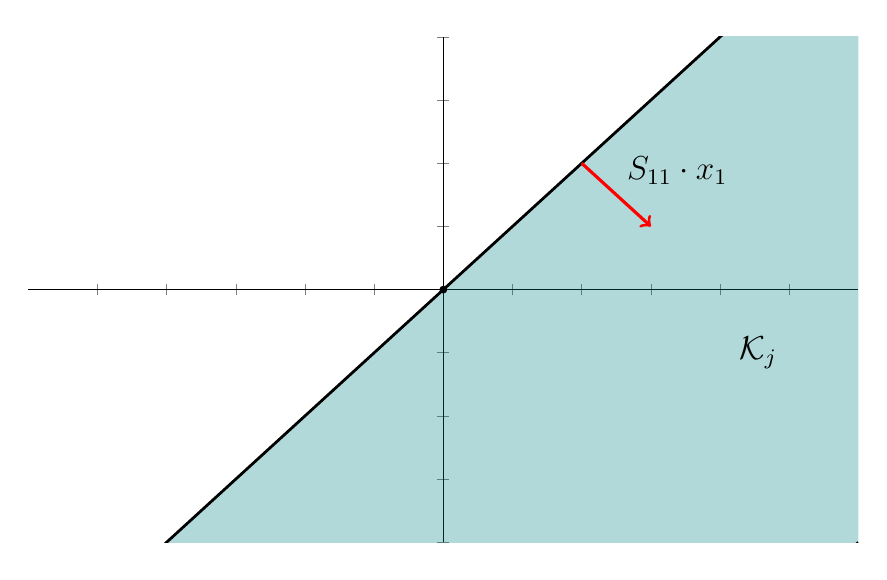
\begin{tikzpicture}[scale=1,
		declare function={
				cone_1(\x)= \x;
				cone_2(\x)= -\x;
				cone_3(\x)= -4*\x;
				bounds(\x)= \x - 10;
			}
	]
	\begin{axis}[width=\linewidth, height=8cm,
			axis lines=center, yticklabels={,,}, xticklabels={,,},
			ymin=-4, ymax=4, ytick={-5,...,5}, ylabel=$$, x axis line style={-},
				xmin=-6, xmax=6, xtick={-5,...,5}, xlabel=$$, y axis line style={-},
		]
		\addplot[name path=cone_1, domain=-6:6, samples=100, line width=1pt]{cone_1(x)};
		%\addplot[name path=cone_2, domain=-6:6, samples=200, line width=1pt]{cone_2(x)};
		%\addplot[name path=cone_3, domain=-6:6, samples=200, line width=1pt]{cone_3(x)};
		\addplot[name path=bounds, domain=-6:6, samples=100, line width=1pt]{bounds(x)};

		% add color fill to both cones.

		\addplot fill between[
				of = cone_1 and bounds,
				%split, % calculate segment
				every even segment/.style = {fill=teal, fill opacity=0.3},
			];

		%% point labels
		% origin point
		\node[circle, fill, inner sep=1pt] at (axis cs:0,0) {};

		% labels
		\node[label={0:$\calK_j$}] at (axis cs:4,-1) {};

		% lines
        \draw [->, draw=red, line width = 0.4mm] (axis cs:2,2) -- (axis cs:3,1) node[midway,above right] {$S_{11} \cdot x_1$};
		%\draw [->, draw=red, line width = 0.4mm] (axis cs:2,-2) -- (axis cs:3,-1) node[midway,below right] {$S_{22} \cdot x_2$};
		%\draw [->, draw=red, line width = 0.4mm] (axis cs:0.5,-2) -- (axis cs:-2.5,-2.75) node[pos=0.9,below right] {$S_{33} \cdot x_3$};
	\end{axis}

\end{tikzpicture}%

	\end{figure}
\end{frame}

\begin{frame}{Cone Decompositions: Proof Sketch}

	\[
		\calK_j'' = \calK_j' \cap \cbr{w : [S_j]_{22} \cdot \abr{x_2, w} \geq 0}
	\]

	\begin{figure}[]
		\centering
		%! TEX root = ../../main.tex

%% Illustration of cone decomposition. 

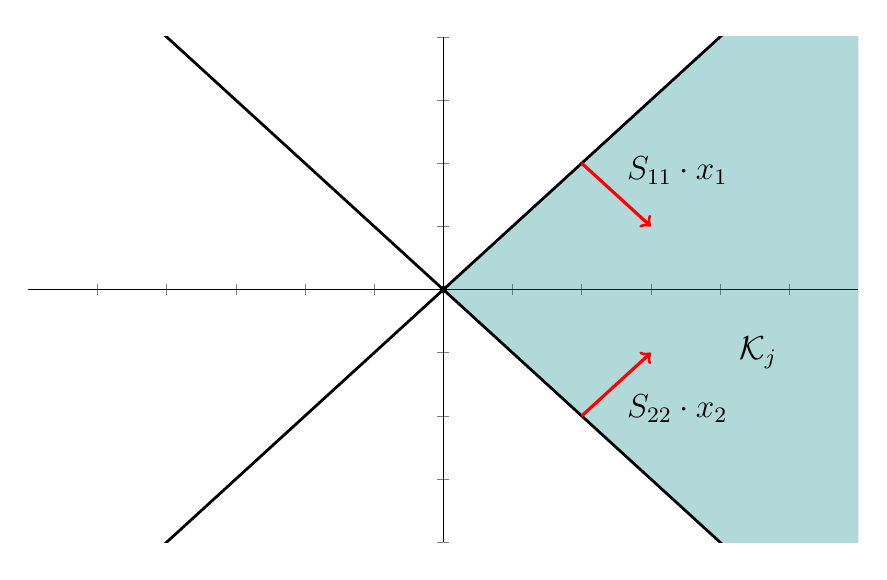
\begin{tikzpicture}[scale=1,
		declare function={
				cone_1(\x)= \x;
				cone_2(\x)= -\x;
				cone_3(\x)= -4*\x;
			}
	]
	\begin{axis}[width=\linewidth, height=8cm,
			axis lines=center, yticklabels={,,}, xticklabels={,,},
			ymin=-4, ymax=4, ytick={-5,...,5}, ylabel=$$, x axis line style={-},
				xmin=-6, xmax=6, xtick={-5,...,5}, xlabel=$$, y axis line style={-},
		]
		\addplot[name path=cone_1, domain=-6:6, samples=100, line width=1pt]{cone_1(x)};
		\addplot[name path=cone_2, domain=-6:6, samples=200, line width=1pt]{cone_2(x)};
		%\addplot[name path=cone_3, domain=-6:6, samples=200, line width=1pt]{cone_3(x)};

		% add color fill to both cones.
		\addplot fill between[
				of = cone_1 and cone_2,
				split, % calculate segments
				every even segment/.style = {fill=blue, fill opacity=0},
				every odd segment/.style  = {fill=teal, fill opacity=0.3}
			];

		%% point labels
		% origin point
		\node[circle, fill, inner sep=1pt] at (axis cs:0,0) {};

		% labels
		\node[label={0:$\calK_j$}] at (axis cs:4,-1) {};

		% lines
        \draw [->, draw=red, line width = 0.4mm] (axis cs:2,2) -- (axis cs:3,1) node[midway,above right] {$S_{11} \cdot x_1$};
		\draw [->, draw=red, line width = 0.4mm] (axis cs:2,-2) -- (axis cs:3,-1) node[midway,below right] {$S_{22} \cdot x_2$};
		%\draw [->, draw=red, line width = 0.4mm] (axis cs:0.5,-2) -- (axis cs:-2.5,-2.75) node[pos=0.9,below right] {$S_{33} \cdot x_3$};
	\end{axis}

\end{tikzpicture}%

	\end{figure}
\end{frame}


\begin{frame}{Cone Decompositions: Proof Sketch}

	\[
		\calK_j''' = \calK_j'' \cap \cbr{w : [S_j]_{33} \cdot \abr{x_3, w} \geq 0}
	\]

	\begin{figure}[]
		\centering
		%! TEX root = ../../main.tex

%% Illustration of cone decomposition. 

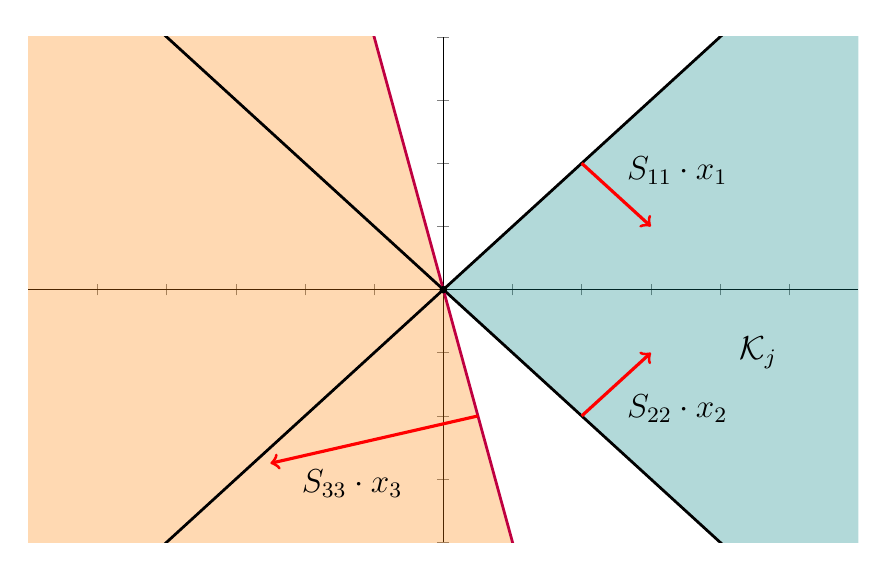
\begin{tikzpicture}[scale=1,
		declare function={
				cone_1(\x)= \x;
				cone_2(\x)= -\x;
				cone_3(\x)= -4*\x;
				bounds(\x)= -4*\x - 100;
			}
	]
	\begin{axis}[width=\linewidth, height=8cm,
			axis lines=center, yticklabels={,,}, xticklabels={,,},
			ymin=-4, ymax=4, ytick={-5,...,5}, ylabel=$$, x axis line style={-},
				xmin=-6, xmax=6, xtick={-5,...,5}, xlabel=$$, y axis line style={-},
		]
		\addplot[name path=cone_1, domain=-6:6, samples=100, line width=1pt]{cone_1(x)};
		\addplot[name path=cone_2, domain=-6:6, samples=200, line width=1pt]{cone_2(x)};
		\addplot[name path=cone_3, domain=-6:6, samples=200, line width=1pt, draw=purple]{cone_3(x)};
		\addplot[name path=bounds, domain=-6:6, samples=200, line width=1pt]{bounds(x)};

		% add color fill to both cones.
		\addplot fill between[
				of = cone_1 and cone_2,
				split, % calculate segments
				every even segment/.style = {fill=blue, fill opacity=0},
				every odd segment/.style  = {fill=teal, fill opacity=0.3}
			];

		\addplot fill between[
				of = cone_3 and bounds,
				every even segment/.style = {fill=orange, fill opacity=0.3},
			];

		%% point labels
		% origin point
		\node[circle, fill, inner sep=1pt] at (axis cs:0,0) {};

		% labels
		\node[label={0:$\calK_j$}] at (axis cs:4,-1) {};

		% lines
        \draw [->, draw=red, line width = 0.4mm] (axis cs:2,2) -- (axis cs:3,1) node[midway,above right] {$S_{11} \cdot x_1$};
		\draw [->, draw=red, line width = 0.4mm] (axis cs:2,-2) -- (axis cs:3,-1) node[midway,below right] {$S_{22} \cdot x_2$};
		\draw [->, draw=red, line width = 0.4mm] (axis cs:0.5,-2) -- (axis cs:-2.5,-2.75) node[pos=0.9,below right] {$S_{33} \cdot x_3$};
	\end{axis}

\end{tikzpicture}%

	\end{figure}
\end{frame}


\begin{frame}{Cone Decompositions: Proof Sketch}

	\[
		\tilde \calK_j''' = \calK_j'' \cap \cbr{w : -[S_j]_{33} \cdot \abr{x_3, w} \geq 0}
	\]

	\begin{figure}[]
		\centering
		%! TEX root = ../../main.tex

%% Illustration of cone decomposition. 

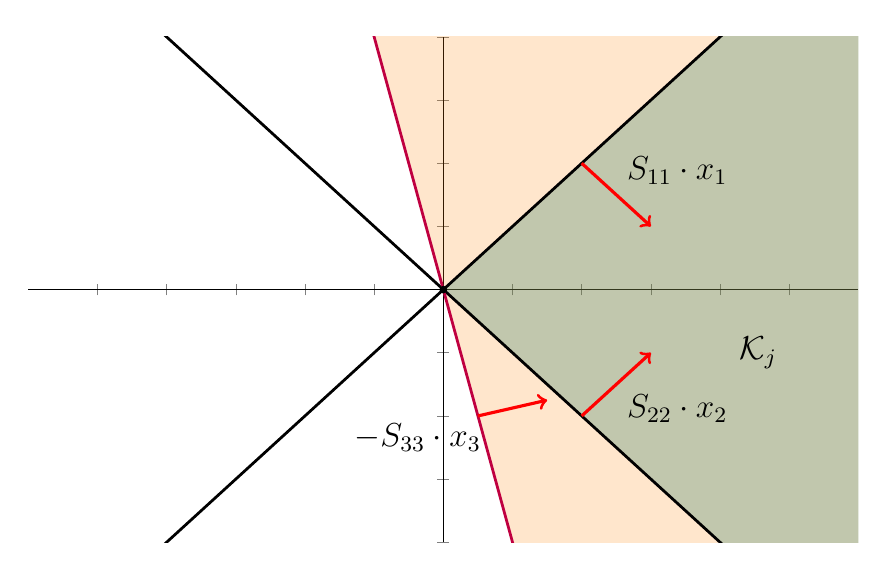
\begin{tikzpicture}[scale=1,
		declare function={
				cone_1(\x)= \x;
				cone_2(\x)= -\x;
				cone_3(\x)= -4*\x;
				bounds(\x)= -4*\x + 100;
			}
	]
	\begin{axis}[width=\linewidth, height=8cm,
			axis lines=center, yticklabels={,,}, xticklabels={,,},
			ymin=-4, ymax=4, ytick={-5,...,5}, ylabel=$$, x axis line style={-},
				xmin=-6, xmax=6, xtick={-5,...,5}, xlabel=$$, y axis line style={-},
		]
		\addplot[name path=cone_1, domain=-6:6, samples=100, line width=1pt]{cone_1(x)};
		\addplot[name path=cone_2, domain=-6:6, samples=200, line width=1pt]{cone_2(x)};
		\addplot[name path=cone_3, domain=-6:6, samples=200, line width=1pt, draw=purple]{cone_3(x)};
		\addplot[name path=bounds, domain=-6:6, samples=200, line width=1pt]{bounds(x)};

		% add color fill to both cones.
		\addplot fill between[
				of = cone_1 and cone_2,
				split, % calculate segments
				every even segment/.style = {fill=blue, fill opacity=0},
				every odd segment/.style  = {fill=teal, fill opacity=0.3}
			];

		\addplot fill between[
				of = cone_3 and bounds,
				every even segment/.style = {fill=orange, fill opacity=0.2},
			];

		%% point labels
		% origin point
		\node[circle, fill, inner sep=1pt] at (axis cs:0,0) {};

		% labels
		\node[label={0:$\calK_j$}] at (axis cs:4,-1) {};

		% lines
        \draw [->, draw=red, line width = 0.4mm] (axis cs:2,2) -- (axis cs:3,1) node[midway,above right] {$S_{11} \cdot x_1$};
		\draw [->, draw=red, line width = 0.4mm] (axis cs:2,-2) -- (axis cs:3,-1) node[midway,below right] {$S_{22} \cdot x_2$};
		\draw [->, draw=red, line width = 0.4mm] (axis cs:0.5,-2) -- (axis cs:1.5,-1.75) node[pos=0.2,below left] {$-S_{33} \cdot x_3$};
	\end{axis}

\end{tikzpicture}%

	\end{figure}
\end{frame}

\begin{frame}{Cone Decomposition: Main Result}
	\begin{itemize}
		\item The real proof is more complex, but this is the core idea.
		      \vspace{0.2em}
		      \begin{itemize}
			      \item Build \( \calK_i \) by switching signs of \( [S_j]_{ii} \).
			            \vspace{0.2em}
			      \item Equivalent to turning on/off activations.
		      \end{itemize}
		      \vspace{0.4em}

		\item Leads to our main approximation result.
	\end{itemize}



	\pause
	\horizontalrule

	\begin{beamercolorbox}[wd=\textwidth,sep=1em]{result}
		\textbf{Theorem 3.7} (informal):
		Let \( \lambda \geq 0 \) and let \( p^* \) be the optimal value of the ReLU problem.
		There exists a C-GReLU problem with minimizer \( u^* \) and optimal value \( d^* \) satisfying,
		\[
			d^* \leq p^* \leq d^* + \textcolor{Red}{2 \lambda \kappa(\tilde X_{\calJ}) \sum_{D_i \in \tilde \calD} \norm{u_i^*}_2}.
		\]
	\end{beamercolorbox}

\end{frame}

\begin{frame}{Cone Decompositions: Big Picture}
	\begin{figure}[]
		\centering
		%! TEX root = ../../main.tex

%% illustration of relations between hypothesis classes. 

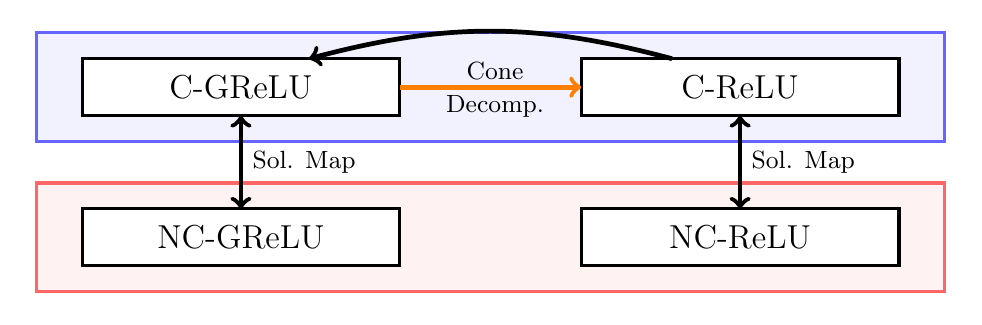
\begin{tikzpicture}[scale=1,
	]
	\begin{axis}[width=1.1\linewidth, height=5cm,
			axis lines=none,  % don't print axis lines
			yticklabels={,,}, xticklabels={,,},
			ymin=-0.2, ymax=10.2, x axis line style={-},
			xmin=-0.2, xmax=20.2, y axis line style={-},
		]

		\filldraw[color=blue!60, fill=blue!5, line width=0.4mm](axis cs:0,5.8) rectangle (axis cs:20, 10);
		\filldraw[color=red!60, fill=red!5, line width=0.4mm](axis cs:0,0) rectangle (axis cs:20, 4.2);

		% non-convex models
		\filldraw[line width=0.4mm, fill=white](axis cs:1,1) rectangle (axis cs:8, 3.2) node[pos=.5] {NC-GReLU};
		\filldraw[line width=0.4mm, fill=white](axis cs:12,1) rectangle (axis cs:19, 3.2) node[pos=.5] {NC-ReLU};

		% convex models
		\filldraw[line width=0.4mm, fill=white](axis cs:1,6.8) rectangle (axis cs:8, 9) node[pos=.5] {C-GReLU};
		\filldraw[line width=0.4mm, fill=white](axis cs:12,6.8) rectangle (axis cs:19, 9) node[pos=.5] {C-ReLU};

		\draw [<->, solid, draw=black, line width = 0.6mm] (axis cs:4.5,3.2) -- (axis cs:4.5,6.8) node[right, pos=0.5] {\small Sol. Map};

		\draw [<->, solid, draw=black, line width = 0.6mm] (axis cs:15.5,3.2) -- (axis cs:15.5,6.8)  node[right, pos=0.5] {\small Sol. Map};

        \draw [<-, solid, draw=black, line width = 0.6mm] (axis cs:6,9) to [bend left=15] (axis cs:14, 9);

		\draw [->, solid, draw=orange, line width = 0.6mm] (axis cs:8,7.9) -- (axis cs:12,7.9);
		\node[align=center] at (axis cs:10.1, 7.8) {\small Cone\\ \small Decomp.};
	\end{axis}

\end{tikzpicture}%

	\end{figure}
	\pause

	\textbf{Takeaways}:

	\vspace{0.5em}
	\begin{itemize}
		\item Gated ReLU and ReLU model classes are the same.
		\item We can convert between them at will.
	\end{itemize}
\end{frame}

\setbeamercolor{background canvas}{bg=LightCyan}

\begin{frame}{}
	\begin{center}
		\huge IV. Algorithms
	\end{center}
\end{frame}
\setbeamercolor{background canvas}{bg=white}

\begin{frame}{Algorithms: ReLU by Cone Decomposition}
	\begin{center}
		\large Using cone decompositions \textbf{in practice}.
	\end{center}

	\pause
	\horizontalrule

	\begin{enumerate}
		\item Solve the gated ReLU problem:
		      \[
			      u^* \in \argmin_{u} \norm{\sum_{j=1}^p D_j X u_j - y}_2^2 + \lambda \sum_{j=1}^p \norm{u_j}_2
		      \]
		      \pause
		\item Solve a cone decomposition:
		      \[
			      v_j^*, w_j^* \in \argmin_{v_j, w_j} \cbr{ L(v_j, w_j) : v_j - w_j = u^*_j}
		      \]
		      \pause

		\item Compute corresponding ReLU model.
	\end{enumerate}

\end{frame}

\begin{frame}{Algorithms: Solving the Convex Programs}
	We develop two algorithms for solving the convex reformulations:

	\vspace{1em}

	\begin{itemize}
		\item \textbf{R-FISTA}: a restarted FISTA variant for Gated ReLU.
		      \vspace{0.5em}
		\item \textbf{AL}: an augmented Lagrangian method for the (constrained) ReLU Problem.
	\end{itemize}

	\pause
	\horizontalrule

	And we can use all the convex tricks!
	\vspace{1em}
	\begin{itemize}
		\item \textbf{Fast}: \( O(1/T^2) \) convergence rate.
		      \vspace{0.5em}

		\item \textbf{Tuning-free}: line-search, restarts, data normalization, \ldots
		      \vspace{0.5em}

		\item \textbf{Certificates}: termination based on min-norm subgradient.
	\end{itemize}

\end{frame}

\begin{frame}{Algorithms: Completing the Picture}
	\begin{center}
		\Large
		Returning to our first example...
	\end{center}

	\begin{figure}[]
		\centering
		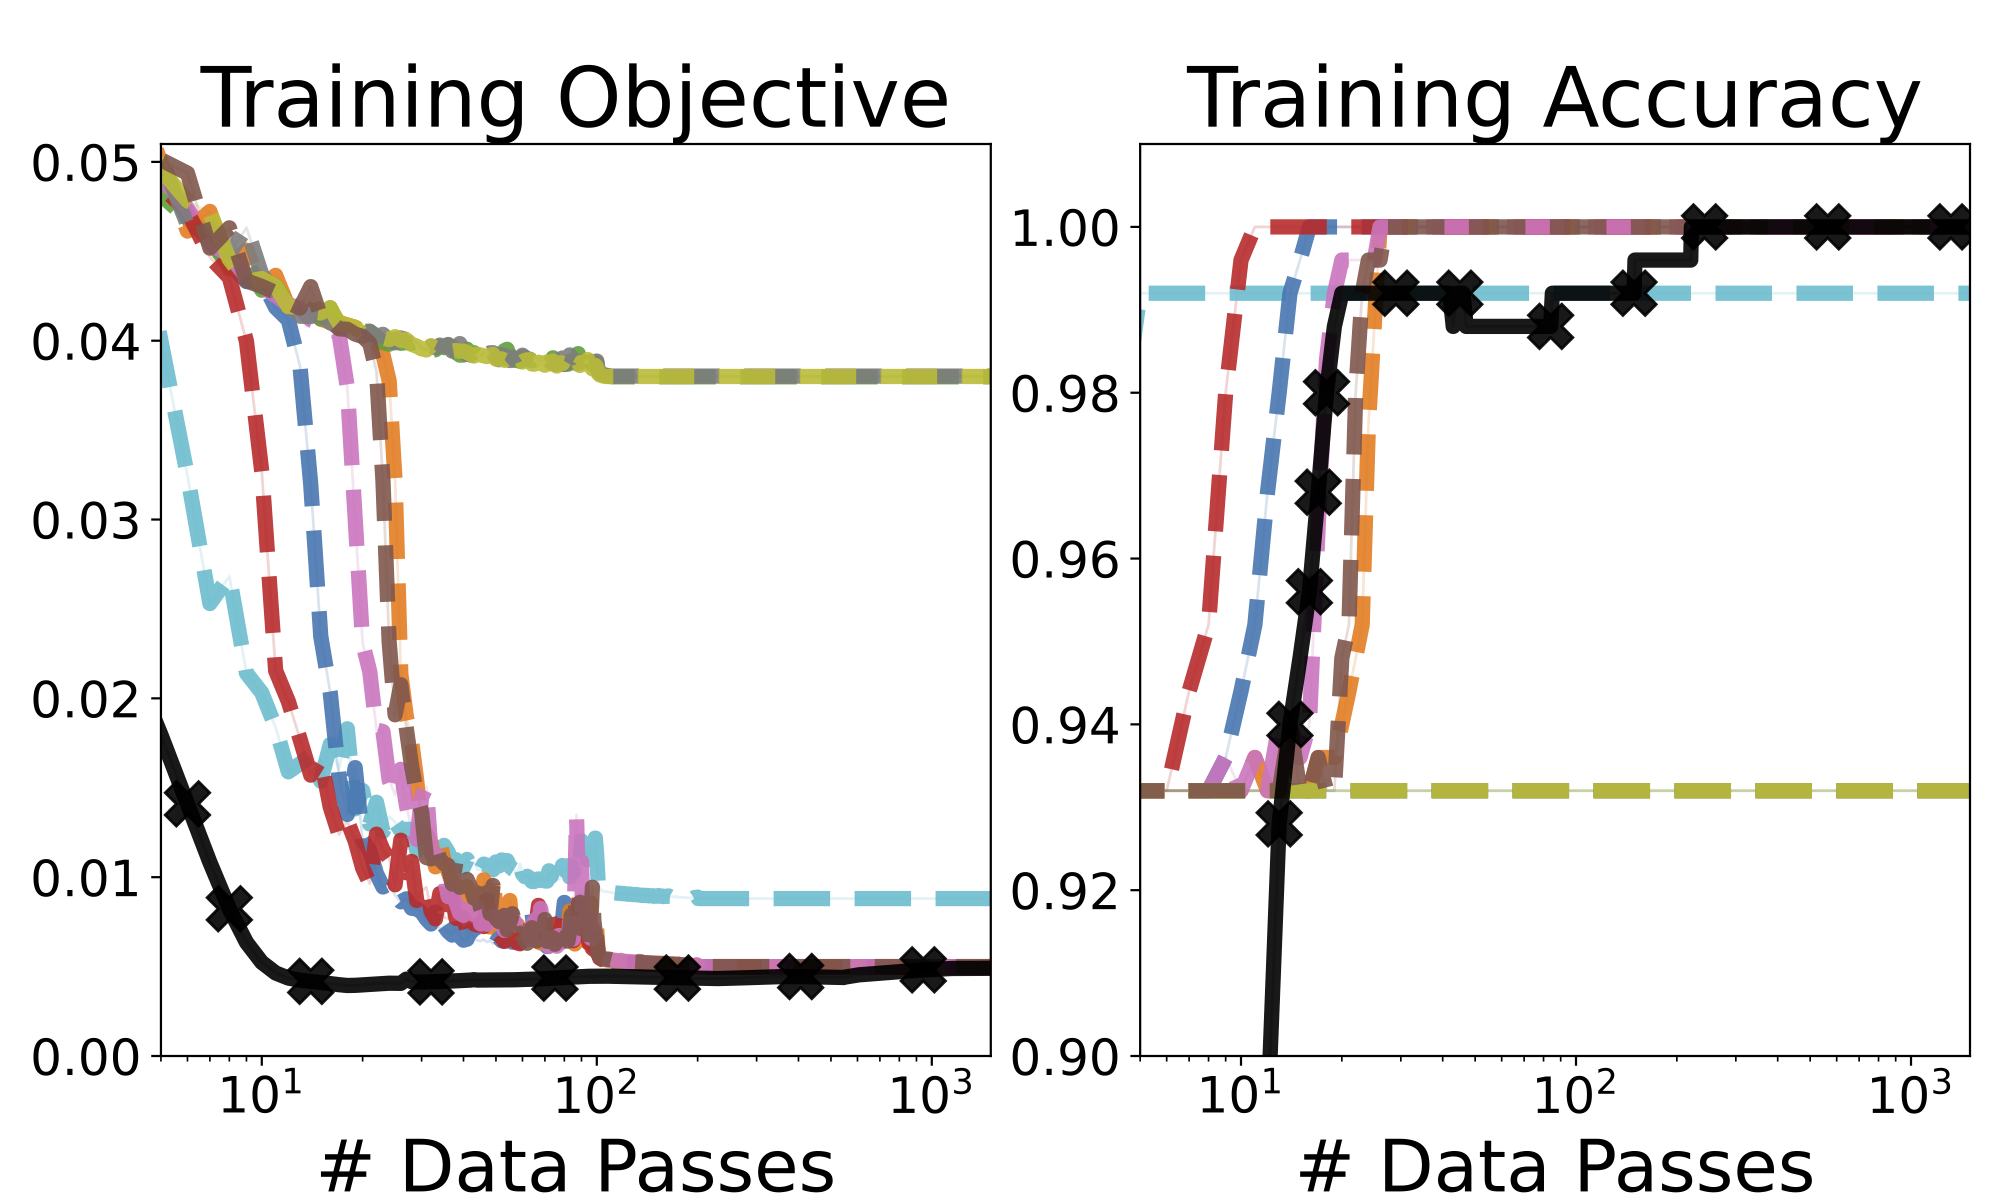
\includegraphics[width=0.9\textwidth]{assets/synthetic_classification.png}
	\end{figure}
\end{frame}

\begin{frame}{Algorithms: Large-Scale Robustness}
	\begin{figure}[t]
		\centering
		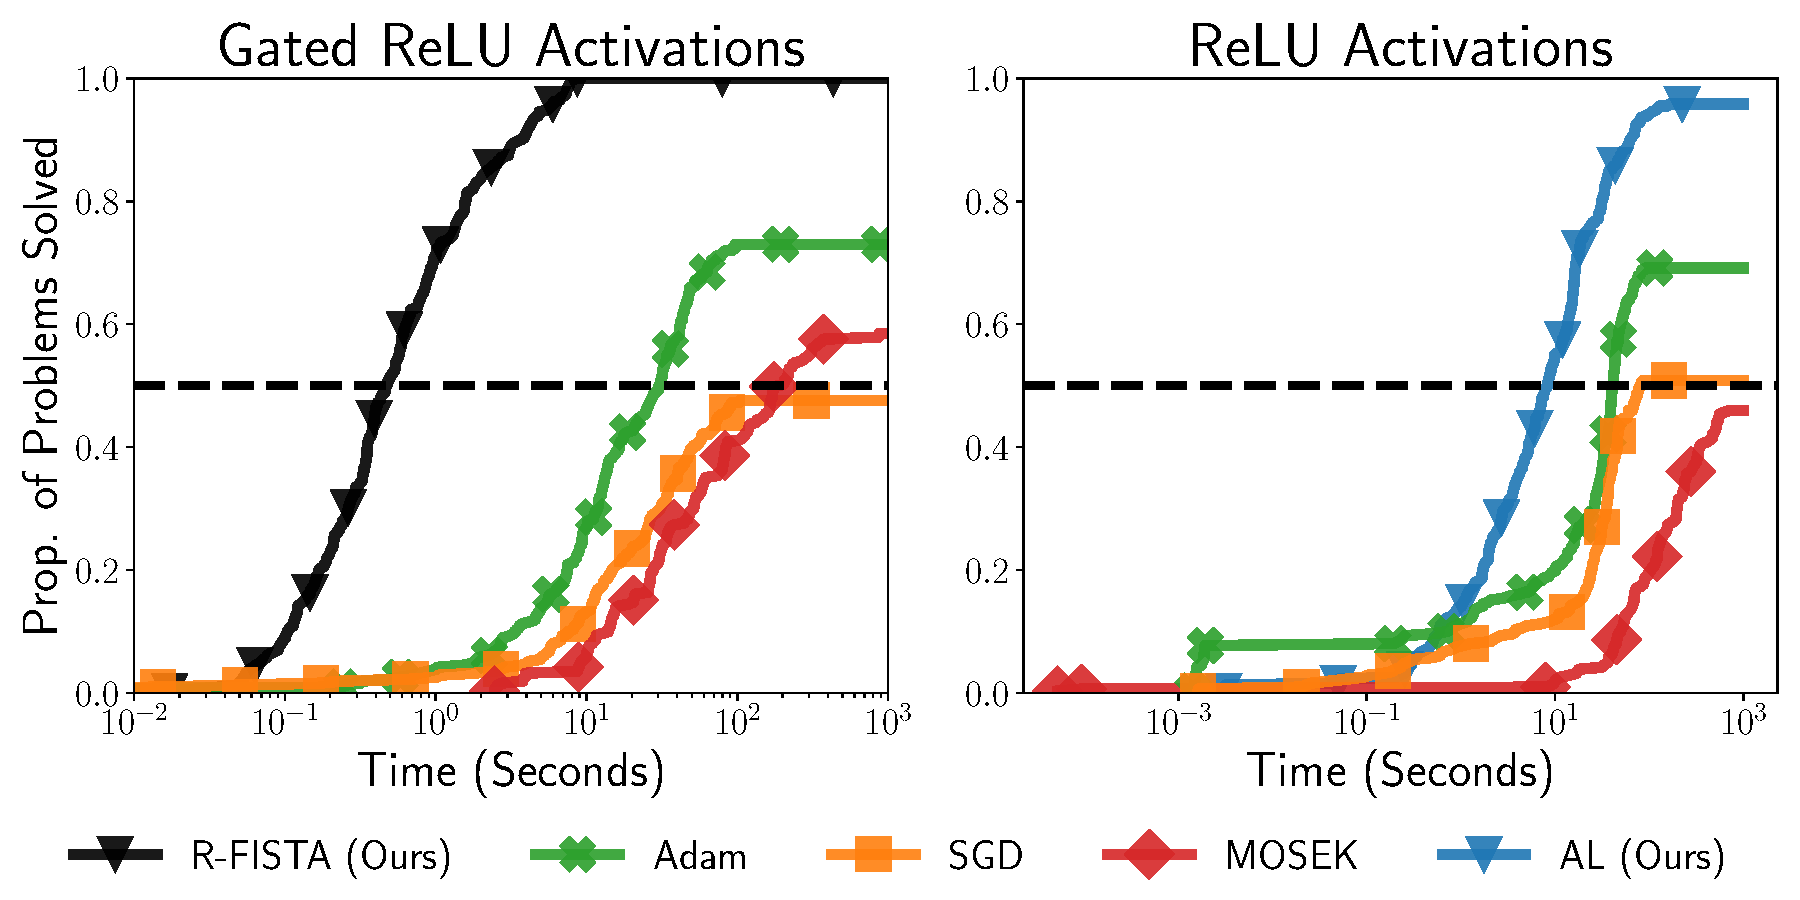
\includegraphics[width=1\linewidth]{assets/pp_main.pdf}
	\end{figure}
	\begin{itemize}
		\item Generated by 438 training problems taken from UCI repo.
		\item R-FISTA/AL solve more, faster, than SGD and Adam.
	\end{itemize}
\end{frame}

\setbeamercolor{background canvas}{bg=LightCyan}

\begin{frame}{}
	\begin{center}
		\huge Pause.
	\end{center}
\end{frame}
\setbeamercolor{background canvas}{bg=white}

\begin{frame}{Recap}
	\begin{center}
		\huge   Our Contributions.
	\end{center}

	\vspace{2em}
	\pause
	{ \large
		\begin{itemize}
			\item We develop new convex reformulations of two-layer neural networks
			      with \textbf{gated ReLU} activations.\pause
			      \vspace{0.5em}

			\item We  approximate the ReLU training problem by \textbf{unconstrained}
			      convex optimization of a Gated ReLU network.\pause
			      \vspace{0.5em}

			\item We propose and \textbf{exhaustively evaluate} algorithms for solving
			      our convex reformulations.
		\end{itemize}
	}

\end{frame}


%% main content ends %%

%% end slide
\setbeamercolor{background canvas}{bg=LightCyan}

\begin{frame}{}
	\begin{center}
		\huge Try our Code!
	\end{center}

	\begin{figure}[]
		\centering
		
\includegraphics[width=0.6\textwidth]{assets/github.png}
	\end{figure}
\end{frame}
\setbeamercolor{background canvas}{bg=white}

%% bibliography
\begin{frame}[allowframebreaks]{References}
	\printbibliography[]
\end{frame}


\end{document}
